\chapter{Реактивни средства}
\label{ch:reactive-tools}

\section{Събитиен вход/изход. Шаблони \emph{реактор} и \emph{проактор}}

Важен аспект на приложенията е комуникацията им с външни системи и компоненти. За тази цел много приложения използват блокиращи операции за вход и изход. В тази секция ще разгледаме подходи, базирани на вход и изход чрез събитийни съобщения.

\subsection{Шаблон \emph{реактор}}
\label{sec:reactor-pattern}

Първият подход, който ще разгледаме, се нарича \emph{реактор}. Той позволява комуникацията по няколко входно/изходни канала да бъде извършвана чрез една нишка. Описан е от Дъглас Шмид в негова научна публикация от 1995-та година \cite{schmidt1995Reactor}.

Един реактор се състои от следните компоненти \cite{schmidt1995Reactor}:

\begin{itemize}
  \item \emph{Ресурсен идентификатор} (\englishterm{Handler}) — обект, идентифициращ комуникационен канал или друг ресурс, който асинхронно генерира събития, означаващи готовност дадена операция да бъде извършена. Такива събития могат да бъдат заявка за осъществяване на връзка, получени данни за четене, готовност за писане и други.
  
  \item \emph{Синхронен събитиен демултиплексор} — компонент, предоставящ функционалност за следене на група от ресурси за събития върху тях. Той предоставя интерфейс за извличане на необработени събития, който при липса на такива блокира текущата нишка до възникване на нови. Възникването на събитие означава, че е \emph{възможно да бъде извършена съответната операция без да бъде блокирана текущата нишка}.
  
  Събитийният демултиплексор най-често се имплементира от операционната система, която и управлява съответните ресурси. Такива имплементации са системните примитиви \code{epoll}, \code{kqueue}, \code{select} и други в съвременните операционни системи.
  
  \item \emph{Събитиен наблюдател} (\englishterm{Event handler}) — интерфейс за обекти с програмна логика, които да бъдат активирани при възникване на определено събитие. Заедно с конкретните наблюдатели и ресурсите са имплементация на шаблона \emph{наблюдател}.
  
  \item \emph{Конкретен събитиен наблюдател} (\englishterm{Concrete event handler}) — конкретна имплементация на събитиен наблюдател, съдържащ логика, която да бъде изпълнена при възникване на определени събития върху конкретен ресурс.
  
  \item \emph{Иницииращ диспечер} — управлява регистрирането и премахването на събитийни наблюдатели за определени ресурс и събития и реализира извикването им при възникване на конкретните събития. За целта използва събитийния демултиплексор, обикновено в цикъл, наречен \emph{събитиен цикъл}. Това е централният компонент на една реактор имплементация.
\end{itemize}

\begin{figure}
  \centering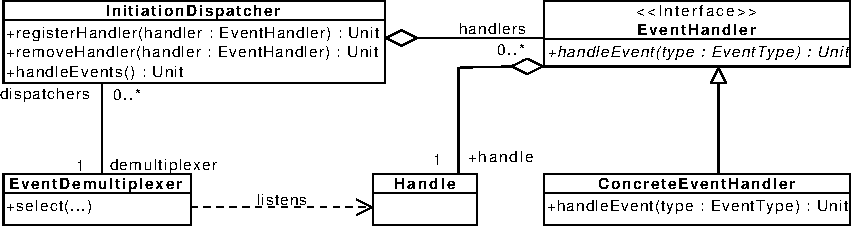
\includegraphics[width=\textwidth]{images/reactor.pdf}
  \caption{Връзки между компонентите на един реактор}
  \label{fig:reactor-components}
\end{figure}

\shortlabeledref{Фигура}{fig:reactor-components} представя връзките между тези компоненти.

Нека да напишем имплементация на реактор. Ще използваме Java библиотеката \code{java.nio}, която предоставя реализация на няколко вида канала и на събитиен демултиплексор. Библиотеката използва съответните системни примитиви и структури на операционната система.

Пакетът \code{java.nio} предоставя няколко типа комуникационни канала. Това са \code{FileChannel} за файлове, \code{SocketChannel} за TCP връзки, \code{ServerSocketChannel} за приемане на входящи TCP връзки, \code{DatagramChannel} за UDP комуникация и \code{Pipe} за еднопосочна междунишкова комуникация. От тях \code{FileChannel} не може да бъде използван с демултиплексора, тъй като повечето операционни системи не поддържат това. За останалите е необходимо при създаването си да бъдат настроени в специален неблокиращ режим.

Java поддържа четири различни операции за каналите със съответните им събития. Това са приемане на нова входяща връзка (\englishterm{accept}), осъществяване на изходяща връзка (\englishterm{connect}), четене на данни (\englishterm{read}) и запис на данни (\englishterm{write}).

Класът \code{Selector} имплементира събитийния демултиплексор. Всеки канал може да бъде регистриран в дадена негова инстанция за определени събития. Резултатът от регистрацията е обект от тип \code{SelectionKey}, през който могат да бъдат променяни събитията, за които се отнася регистрацията, и чрез който тя може да бъде премахната.

За имплементация на събитийните наблюдатели бихме могли да използваме функция, която да бъде регистрирана за определена операция, или обект, имплементиращ поведение за всяка една от операциите. Тъй като операциите най-често са взаимно свързани ще използваме втория подход, декларирайки интерфейс за тях, но дефинирайки празна операция по подразбиране.

Иницииращият диспечер ще е компонента, който ще навърже целия реактор. Нека да видим имплементация чрез така разгледаните компоненти.

\lstinputlisting[
  style=listing,
  caption={Имплементация на реактор}
]{../source/reactor-proactor/src/reactor/basic/Reactor.scala}

Всички събитийни наблюдатели трябва да наследяват класа \code{Handler}. Той дефинира методи с логика за всяка от операциите (с празна имплементация), метод за извличане на свързания с него ключ (\code{SelectionKey} обект), от където могат да бъдат извлечени каналът и селекторът, и метод \code{cleanup} за изчистване на регистрацията и на евентуално допълнително състояние на наблюдателя.

Класът \code{CloseOnIOError} е специален клас, който наблюдателите могат да наследят за улесняване на затваряно на канала и на изчистването на ресурсите при възникване на грешка (като \code{IOException}).

\begin{figure}[h]
  \centering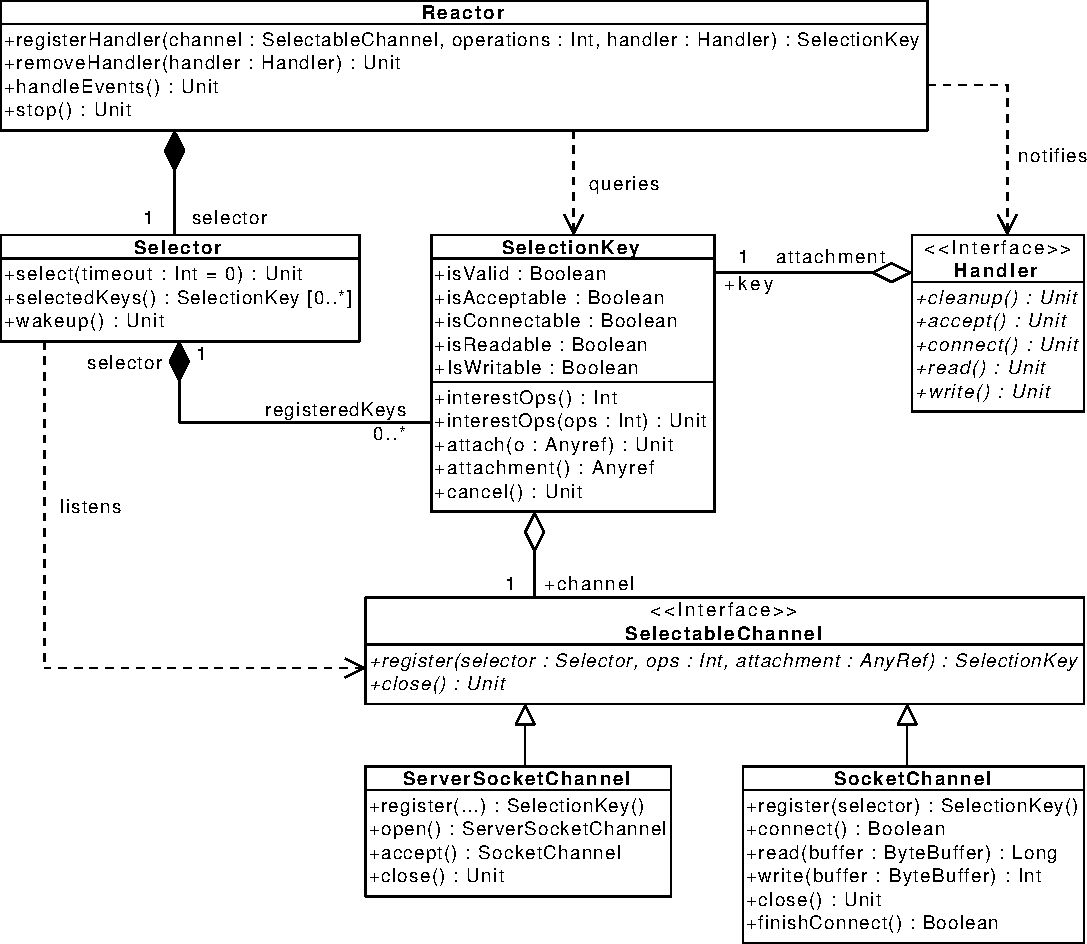
\includegraphics[width=\textwidth]{images/reactor-implementation.pdf}
  \caption{Компоненти на имплементацията на реактор}
  \label{fig:reactor-implementation-components}
\end{figure}

Иницииращият диспечер е реализиран чрез класа \code{Reactor}. Той предоставя методи за регистрация на канал в създадения от него селектор, за премахване на наблюдател и за спиране на реактора. Спирането на реактора може да бъде извършено от всяка друга нишка, което бива подсигурено чрез \lstinline[language=Java]{volatile} променлива. Основният метод \code{handleEvents} е мястото, където се извършва събитийният цикъл. На всяка итерация той блокира текущата нишка до възникване на събития (ред 52). Методът \code{select} приема максимално време, до което да блокира, като 0 съответства на неограничено време. След връщане от \code{select} той обхожда всички ключове, които имат събитие, и извиква съответните функции от техните наблюдатели (редове от 55 до 64). Наведнъж би могло да бъдат генерирани няколко типа събития. Ако някоя от обработващите функции хвърли изключение, то бива прихванато от реактора, а съответният наблюдател премахнат. Без тази защита грешка във всеки един наблюдател може да доведе до срив на целия реактор. Списъкът, върнат от метода \code{preSelectJobs}, ни позволява по-късно да разширим имплементацията с допълнителна функционалност. \shortlabeledref{Фигура}{fig:reactor-implementation-components} показва основните функции на компонентите на имплементацията и връзките между тях.

Нека да реализираме ехо сървър чрез този реактор. Логиката на един сървър, имплементиран чрез реактор, заедно със съответния му наблюдател, приемащ връзки, би била универсална, затова ще я отделим в преизползваеми компоненти. В следващите листинги ще изпускаме \code{import} клаузите:

\lstinputlisting[
  style=listing,
  firstline=8,
  caption={Имплементация на приемател на TCP връзки}
]{../source/reactor-proactor/src/reactor/basic/acceptor/CommonAcceptor.scala}

\lstinputlisting[
  style=listing,
  firstline=10,
  caption={Имплементация на сървър чрез реактор}
]{../source/reactor-proactor/src/reactor/basic/server/SingleReactorServer.scala}

\lstinputlisting[
  style=listing,
  firstline=8,
  caption={Наблюдател за ехо сървър}
]{../source/reactor-proactor/src/reactor/EchoHandler.scala}

\lstinputlisting[
  style=listing,
  firstline=5,
  caption={Имплементация на ехо сървър}
]{../source/reactor-proactor/src/reactor/EchoServer.scala}

Сървърът използва текущата нишка (в случая главната нишка) за да стартира цикъла на диспечера, регистрирайки приемащ наблюдател за сървър на порт 8000. При нова връзка се създава нова инстанция на \code{EchoHandler} (ред 6 от \code{CommonAcceptor}), която обработва връзката до нейното затваряне (ред 9 от \code{EchoHandler} или при грешка). Една единствена нишка обработва абсолютно всички ехо връзки до сървъра, като връзките съществуват паралелно.

\code{EchoHandler} използва специален обект \code{ByteBuffer}, в който биват съхранявани прочетените данни, което бива последвано от тяхното записване обратно в канала. Всеки \code{ByteBuffer} има капацитет, като \code{read} операцията запълва само оставащите байтове от буфера, докато той не бъде изпразнен. Боравенето с \code{ByteBuffer} е свързано с доста изменяеми операции, което прави работата с него трудна и податлива на грешки. Затова ще изолираме този обект само в наблюдателите и по възможност ще използваме функционален код с минимална изменяемост в останалата част от програмата. Можем да забележим, че \code{EchoHandler} се регистрира за операция за писане само когато има данни, които да запише. В противен случай, при постоянна регистрация, неговия \code{write} метод ще бъде излишно извикван на всяка итерация на сибитийния цикъл. Аналогично, ако при \code{read} не са били прочетени всички данни, на следващата итерация методът ще бъде извикан отново. Събитието гарантира, че при четене ще бъде прочетен поне един байт от канала без \code{read} операцията да блокира.

\subsubsection{Ползи и особености на реактора}

Основното свойство на реактор шаблона е, че позволява входно/изходни операции към множество канали да бъдат извършвани без блокиране. При блокиращия вход/изход е необходима нишка за всеки един канал, когато комуникацията по тях се осъществява паралелно. Това ограничава броя на каналите и броя на клиентите, които един сървър би могъл да обработи едновременно, тъй като, както видяхме в \shortlabeledref{секция}{sec:concurrency-threads-scalability}, нишките са скъп ресурс и големият брой на активни нишки води до забавяне на процесора. Един реактор може да обработва огромен брой паралелни връзки само чрез една нишка. Това е особено полезно когато отдалечената страна е бавна, както и за реализиране на дълготрайни връзки, при които спорадично се предават данни, обикновено в резултат на някакви събития. Така чрез реактор успешно биха могли да бъдат обработвани множество (десетки хиляди) дълготрайни уеб сокет връзки. При блокиращия вход/изход броят на връзките бива ограничен от броя на наличните нишки.

Реакторът позволява приемането на няколко паралелни съобщения наведнъж, под формата на събития. Тези съобщения биват генерирани асинхронно от комуникационните канали. Самите операции са синхронни, но неблокиращи, което позволява практичеки едновременна обработка на всички едновременно възникнали събития. В \shortlabeledref{секция}{sec:proactor-using-reactor-messaging} ще видим как можем да направим тези събития явни съобщения и да реализираме асинхронното препредаване на данните от техните операции.

Производителността на реактора зависи от имплементацията на съответните системни примитиви в операционните системи. В операционната система Windows имплементацията на събитиен демултиплексор е по-бавна от тази в Линукс. Windows обаче притежава добри примитиви за асинхронен вход/изход (\englishterm{I/O Completion Ports}), които могат да бъдат използвани за шаблона проактор (\shortlabeledref{секция}{sec:proactor}). Съответните на тях версии в Линукс (примитиви aio) все още създават някои проблеми. В съвременните ОС блокиращите операции позволяват малко по-висока пропускливост на данни за единица време от останалите подходи \cite{tyma2008ThousandOfThreads}. Поради ограниченията на нишките обаче те са неподходящи за голям брой връзки. Ако бъде увеличен броят на нишките това води до увеличено превключване на контекста и забавяне на пропускливостта. Истинската ползва на реактора (и проактора) е възможността за обработка на много клиенти. В \shortlabeledref{секция}{sec:reactor-proactor-performance} ще видим сравнение на производителността на разгледаните подходи.

Някои софтуерни среди изцяло базират своя програмен модел на реактор. Такава е например платформата Node.js. Тя реализира еднонишкова JavaScript среда, при която програмната логика се изпълнява в резултат на възникнали събития и се контролира от събитиен цикъл на реактор. Node.js разширява своя реактор с допълнителни събития. Това е например имплементацията на JavaScript функцията \code{setTimeout}. Лесно можем да добавим поддръжка на това и в нашия реактор:

\lstinputlisting[
  style=listing,
  firstline=7,
  caption={Имплементация на реактор с таймаут операция}
]{../source/reactor-proactor/src/reactor/basic/TimeoutReactor.scala}

Реализацията използва подхода за декориране на методи чрез \code{trait} класове на Scala за да добави задачи към списъка \code{preSelectJobs}. Интерфейса на реактора се разширява с метод за регистриране на операция, която да бъде изпълнена след определено време. Операцията се подава по име, което позволява нейното изпълнение да бъде отложено и скрито във функция. Таймаута се реализира използвайки таймаут параметъра на \code{select} функцията. На всяка итерация на събитейния цикъл той бива блокиран най-много за времето, оставащо до следващата операция. Нов реактор с тази функционалност би бил създаден чрез \code{new Reactor with TimeoutReactor}.

Системите, базирани на реактор, предоставят много друга функционалност, която стъпва на вход/изхода от реактора и го скрива, директно имплементирайки различни протоколи. Такива са например опростена функционалност за комуникация по TCP канали, за извършване на заявка към външна услуга по HTTP протокол, за комуникация с базата от данни и много други. По конвенция Node.js използва \englishterm{callback функции} за обратна връзка с бизнес логиката.

Можем да забележим, че боравенето с досега описания реактор изисква много \englishterm{callback} функции от тип \code{T => Unit}. Такива са дори методите на събитийните наблюдатели (стандартен начин за реализация на шаблона наблюдател). Това обаче предполага използване на изменяемо състояние и странични ефекти и невъзможност за композиране на различни операции. Именно поради това програмите на Node.js страдат от тежък и трудно-проследим код, свързан с много състояние. За такъв код се използва терминът \englishterm{callback hell}. В следващите секции от тази глава ще видим алтернативи, които прилагат функционален подход за справяне на този проблем. Ще разгледаме монадни структури, като \code{Future} и асинхронни потоци, които скриват изменяемостта на реактора зад чист функционален код.

Системите като Node.js са по-неустойчиви. При тях цялата бизнес логиката на приложението бива изпълнявана в една и съща нишка с реактора, поради което е доста по-вероятно да бъде генерирана неочаквана грешка. Затова при имплементация на реактор е необходимо предпазване от изключение на всички места, при които се изпълнява клиентки код. Грешки, които водят до прекъсване на текущата нишка, обаче няма как да бъдат предотвратени. Допълнително, ако бизнес логиката използва блокиращи операции или код, извършващ значителни изчисления, това ще блокира реактора и той няма да може да обработва други връзки. Така Node.js е неустойчива среда. В \shortlabeledref{секция}{sec:proactor-using-reactor-messaging} ще видим как да изведем бизнес логиката в отделни нишки и да използваме асинхронни съобщения за препредаване на събитията от реактора.

Друго ограничение на реактор шаблона е, че една нишка утилизира само едно ядро на съвременните многоядрени процесори. Шаблонът обаче няма външно състояние, което позволява той много лесно да бъде скалиран и репликиран на няколко ядра. В \shortlabeledref{секция}{sec:multi-reactor-server} ще разгледаме подход за имплементиране на сървър чрез множество реактори.

\subsubsection{Използване на вход/изход, наличен само чрез блокиращи операции}

Както споменахме, някои операции, като работата с файлове, е възможно да са налични само под блокираща форма в операционната система. Би било добре обаче техния вход/изход също да минава през абстракцията на реактора. За да не блокираме нишката на реактора, един подход би бил да използваме отделно множество от нишки, предназначено само за блокиращи операции. Тъй като съвременните твърди дискове и други персистентни устройства могат да обработват ограничен брой паралелни задачи, то броят на тези нишки не е нужно да бъде голям, за да бъде използвано устройството оптимално. Една заявка за файл или би била ограничена от производителността на устройството или, ако файлът вече е кеширан в операционната система, тя би завършила веднага без блокиране. След завършване на операцията чрез междунишкова комуникация информацията от нея може да бъде изпратена на реактора, който да я обработи като подходящ тип събитие. Начин за реализиране на междунишковата комуникация с реактора ще видим в \shortlabeledref{секция}{sec:multi-reactor-server}.

Съвременните уеб сървъри, базирани на реактор, като Nginx използват такъв подход за работа с файлове, като кешират информацията за да бъде ограничен бавния достъп до тях. Node.js също реализира такова множество от нишки.

\subsubsection{Използване на машини на крайните състояния за контролиране на страничните ефекти при реактор}

Ще отбележим интересна особеност на системите, ориентирани около събития и съобщения. Събитията, като обекти, много естествено се вписват като вход в математическите \emph{машини на крайните състояния} (крайни автомати). Доста често обработката на вход/изход може да бъде описана именно чрез такава абстракция. Всяко получаване на събития представлява нов вход в машината, като тя „реагира“ на него и изменя своето състояние. Така математически можем да ограничим страничните ефекти до точно определени, които да бъдат следени лесно. Актьорите от актьорският модел, който ще разгледаме в секция 4.3, също много естествено могат да моделират краен автомат, тъй като са ориентирани около съобщения.

Чрез реакторен вход/изход обработката на протоколи лесно може да бъде представена като краен автомат. Ще разгледаме такава имплементация за парсване на HTTP съобщения (заявка и отговор) в \labeledref{секция}{sec:implementing-a-web-server}. Можем да дефинираме първоначална версия на интерфейс за такъв тип парсъри:

\begin{lstlisting}[
  style=listing,
  caption={Интерфейс на парсър като краен автомат}
]
trait Parser[I, O] { self =>
  private var currentState = process _
  private var pendingInput: Option[I] = None

  protected def process(input: I): Option[O]

  protected def become(state: I => Option[O]): Unit = currentState = state

  protected def becomeAndReceive(input: I)(state: I => Option[O]) = {
    become(state)
    pendingInput = Some(input)
    None
  }

  def receive(input: I): Option[O] = ???

  def >>[M](other: Parser[O, M]): Parser[I, M] = new Parser[I, M] {
    def process(input: I): Option[M] = self.receive(input) match {
      case Some(output) => other.receive(output)
      case None => None
    }
  }
}
\end{lstlisting}

Чрез метода \code{receive} се приема нов вход. Входът води до евентуална промяна на състоянието. При достигане до край (до крайно състояние) се връща изход \code{Some[O]}, а в противен случай \code{None}. Методът \code{process} определя началното състояние. При приемане на вход всяко едно състояние може да реши да премине към друго чрез метода \code{become}.

Различни парсъри лесно биха могли да бъдат комбинирани заедно, ако изходът на един съвпада с входа на друг. Операцията \code{>>} извършва това. Така всеки изход на първия служи за вход на втория.

Повечето библиотеки за асинхронен вход/изход поддържат изграждането на конвейерн от парсъри по такъв начин. Въпреки това тази реализация все още има някои проблеми:

\begin{itemize*}
  \item когато вход се предава на големи парчета от данни с цел оптимизация (например масиви от байтове) е възможно да се достигне резултат преди консумация на цялото парче. За обработка на останалата част от него в текущата имплементация е необходимо или тя да бъде връщана като изход (което затруднява имплементациите) или подадения вход да помни докъде е консумиран, което може да доведе до неочаквани странични ефекти;
  
  \item въпреки ограниченията все пак определени странични ефекти са налични;
  
  \item нивото на композитност е ограничено.
\end{itemize*}

В \labeledref{секция}{sec:reactive-streams} ще разгледаме как можем да се справим с тези проблеми, използвайки абстракции за автомати, които са функционални и неизменяеми и предоставят висока степен на композитност и преизползваемост.

\subsection{Използване на процесорните ядра чрез множество реактори}
\label{sec:multi-reactor-server}

Един сървър се състои от един или малък брой входни канали \code{ServerSocketChannel}. За да се възползваме от всички ядра на процесора ще създадем по един реактор за всяко ядро, като реакторите трябва да могат да си разпределят връзки от каналите. Това може да стане по различни начини. Един вариант е всеки един реактор да се регистрира за сървърния канал. Така обаче при пристигане на нова връзка събитието за това ще бъде получено от всички реактори, като те ще бъдат събудени и ще направят опит за получаване на връзката. Това изисква синхронизация между тях, което е източник на непаралелизуема част в програмата и критична точка\footnote{В действителност всяка операция до канал в имплементацията на Java води до заключване на няколко мютекса, което е излишно ако той се ползва от само една нишка. Както видяхме в \shortlabeledref{секция}{sec:concurrency-threads-scalability} това заключване е сравнимо с CAS операция. Това е така, защото при липса на конкурентност за заключване и отключване в действителност е необходима само CAS операция, без да се превключва до ядрото. При конкурентност на няколко нишки обаче това води до постоянни превключвания и огромно забавяне.}. Само един от тях реално ще получи връзката. Като алтернатива новите версии на ядрото на Линукс поддържат опция за балансиране на връзките между демултиплексорите (\code{SO_REUSEPORT}). Линукс ще уведоми само един от тях за новата връзка. Това обаче не се поддържа от другите ОС и съответно и от Java.

Ще използваме различен подход, при който, освен реактори за всяко ядро, които ще наречем работници, ще имаме и главен реактор, който ще приема връзките и ще препраща всяка от тях към някой от реакторите за да бъде обработена от него. За целта ще бъдат необходими средства за междунишкова комуникация.

\subsubsection{Гарантиране на видимост между нишки}

Както видяхме в \shortlabeledref{секция}{sec:concurrency-threads-scalability} за съгласуването на променливи между нишки в Java е необходимо те да бъдат \lstinline[language=Java]{volatile} (и евентуално обновявани през CAS) или да бъде използвана синхронизация. Какво се случва обаче когато тези променливи са съставни или промяната им води до достъп до други споделени ресурси на нишките? Трябва ли те и всички полета на съставните обекти също да бъдат \lstinline[language=Java, breaklines=false]{volatile}/синхронизирани? Java версия 5 решава този проблем като явно специфицира своя модел на паметта. Спецификацията дефинира релация \emph{случва-се-преди(a, b)} (накратко $hb(a, b)$) върху събития $a$ и $b$, която има следните свойства \cite[секция 17.4.5]{gosling2015JLS8}:

\begin{itemize*}
  \item ако $a$ и $b$ са действия на една и съща нишка, то $hb(a, b)$ ако $a$ е преди $b$ в програмния ред (в реда на изпълнение на операции в нишката);
  \item запис на \lstinline[language=Java]{volatile} променлива \emph{се случва преди} всички последващи нейни четения;
  \item отключването на мютекс \emph{се случва преди} всяко последващото заключване на мютекса;
  \item операцията е транзитивна.
\end{itemize*}

Транзитивността на операцията гарантира, че четенето на \lstinline[language=Java]{volatile} променлива от една нишка позволява нишката да види всички промени, направени от друга нишка, преди другата нишка да запише стойност в тази \lstinline[language=Java]{volatile} променлива. Това ни позволява видимостта на данните между нишки да бъде съгласувана само чрез една \lstinline[language=Java]{volatile} променлива. Това е изключително полезно свойство, което ще видим в действие при имплементацията и на следващите конкурентни абстракции, които ще разгледаме.

За имплементация на комуникацията между реактори ще използваме неблокиращата конкурентна опашка \code{ConcurrentLinkedQueue}, която използва именно CAS операции (които са винаги с \lstinline[language=Java]{volatile} променливи), чрез които гарантира, че добавяне на елемент в опашката \emph{се случва преди} извличане на елемента от нея.

\subsubsection{Имплементация}

Нека добавим нова функционалност на реактора, която му позволява той да приема операции от други нишки:

\lstinputlisting[
  style=listing,
  firstline=7,
  caption={Реактор, приемащ асинхронно операции от други нишки}
]{../source/reactor-proactor/src/reactor/basic/AsyncOperationReactor.scala}

Подобно на \code{TimeoutReactor} тук дефинираме метод \code{receiveOperation}, който регистрира определена операция. Комуникацията се осъществява чрез \code{ConcurrentLinkedQueue}. След добавяне на операцията в опашката се използва метод, който без блокиране сигнализира на демултиплексора на реактора да се събуди (ред 17). Това става чрез специално събитие, което демултиплексора ще получи асинхронно.

След събуждането си и преди последващото блокиране, реактора ще извлече новите операции от опашката и ще ги обработи в собствената си нишка (метод \code{handleOperations}).

Нека да реализираме приемащия наблюдател на главния реактор:

\lstinputlisting[
  style=listing,
  firstline=8,
  caption={Приемащ наблюдател на главния реактор}
]{../source/reactor-proactor/src/reactor/basic/acceptor/WorkersAcceptor.scala}

При всяко получаване на връзка той на \englishterm{round-robin} принцип избира реактор, който да я обработи. След това приема връзката и изпраща операция към реактора за инициализиране на обработката в неговия контекст (ред 17).

Да реализираме и самия сървър:

\begin{lstlisting}[
  style=listing,
  caption={Сървър с множество реактори}
]
class WorkersServer(port: Int)
                   (handler: (Reactor with AsyncOperationReactor with TimeoutReactor, SocketChannel) => Unit) {
  def start() = {
    val acceptorReactor = new Reactor with AsyncOperationReactor
    val numberOfCores = Runtime.getRuntime().availableProcessors()
    val workerReactors = List.fill(numberOfCores)(new Reactor with AsyncOperationReactor with TimeoutReactor)

    val serverSocket = ServerSocketChannel.open().nonblocking.bind(new InetSocketAddress(port))

    acceptorReactor.receiveOperation(new WorkersAcceptor(acceptorReactor, workerReactors, serverSocket)(handler))

    (acceptorReactor :: workerReactors).foreach { reactor =>
      new Thread(new Runnable {
        def run = reactor.handleEvents()
      }).start()
    }
  }
}
\end{lstlisting}

Сървърът създава един главен реактор и няколко реактори-работници. Техният брой зависи от броя на ядрата на системата. След това той създава \code{WorkersAcceptor} за сървърния канал и стартира всеки от реакторите в собствена нишка.

За реализация на ехо сървър може напълно да преизползваме \code{EchoHandler} класа, който написахме по-рано:

\lstinputlisting[
  firstline=5,
  nolol
]{../source/reactor-proactor/src/reactor/WorkersEchoServer.scala}

\subsection{Шаблон \emph{проактор}}
\label{sec:proactor}

Друг шаблон за събитиен вход/изход е \emph{проактор}. Той също е описан от Дъглас Шмид и др. \cite{pyarali1997Proactor}. При него операционната система (или отделен компонент) проактивно извършва входно/изходните операции, асинхронно от изискващите ги компоненти на потребителските приложения, след което тя уведомява приложението чрез събитие. Шмид и др. описват следните компоненти в един проактор:

\begin{itemize}
  \item \emph{Асинхронни операции} — операция, най-често входно/изходна, която се извършва без блокиране на извикващата нишка, асинхронно от нея. При завършване на операцията извикващите компоненти биват уведомени чрез асинхронно събитие. Тези операции са генерализация на операциите на каналите и ресурсите.
  
  \item \emph{Процесор на асинхронни операции} — приема заявки за асинхронни операции и ги изпълнява. След приключване на операцията делегира уведомяването за това към събитийния диспечер. Често компонента бива имплементиран от операционната система.
  
  \item \emph{Събитиен наблюдател} — интерфейс с програмна логика, която да бъде активирана при завършване на операцията.
  
  \item \emph{Проактивен инициатор} — компонент на приложението, който инициира асинхронна операция. Той посочва операцията, която да бъде извършена, съответния ѝ наблюдател и евентуално събитиен диспечер, който да извърши изпълнението на наблюдателя.
  
  \item \emph{Събитиеен диспечер} (\englishterm{Completion Dispatcher}) — приема събитията за завършени операции и уведобява съответните им наблюдатели (изпълнявайки логиката им).
\end{itemize}

\shortlabeledref{Фигура}{fig:proactor-communication} показва комуникацията между тези компоненти за извършване на една операция \cite{pyarali1997Proactor}.

\begin{figure}
  \centering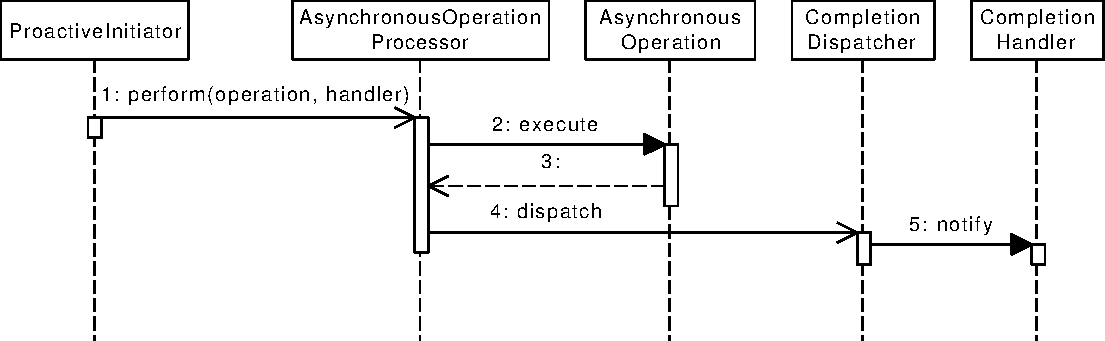
\includegraphics[width=\textwidth]{images/proactor.pdf}
  \caption{Комуникация между компонентите на проактор}
  \label{fig:proactor-communication}
\end{figure}

Java 7 предоставя имплементация на проактор. В библиотеката са дефинирани няколко типа асинхронни канала с техните операции — \code{AsynchronousSocketChannel}, \code{AsynchronousServerSocketChannel} и \code{AsynchronousFileChannel}. Инициирането на операция става през самите канали, като зад тях стои имплементация на \emph{процесора на асинхронни операции}. Под Windows се използва имплементация от ядрото на операционната система (\englishterm{I/O Completion Ports}), а под Линукс бива имплементиран чрез шаблона реактор. Ще видим друга такава имплементация в \shortlabeledref{секция}{sec:proactor-using-reactor-messaging}. Операциите могат да бъдат инициирани асинхронно от всяка една нишка.

Java 7 предоставя интерфейс \code{CompletionHandler} за събитийните наблюдатели, който има два метода — \code{completed} и \code{failed}, в зависимост от резултата от операцията. Сибитийния диспечер е реализиран като множество от нишки, дефинирано от \code{AsynchronousChannelGroup} обект. Всеки канал се обвързва с диспечер при създаването си, като ако такъв не бъде подаден се използва подразбиращ се.

Да разгледаме имплементация на ехо сървър чрез този проактор:

\lstinputlisting[
  style=listing,
  firstline=8,
  caption={Ехо сървър чрез проактор}
]{../source/reactor-proactor/src/proactor/nio/AsyncEchoServer.scala}

Аналогично на реактор имплементацията, тук също имаме \code{Acceptor} и \code{Handler} обекти. В случая единствено отварянето на канала и инициализацията на \code{AsyncAcceptor} се случва в главната нишка, всички останали операции се инициират от множеството от нишки на диспечера (ред 44), в резултат на събитие за завършена операция. За разлика от реактор имплементацията тук събитийната регистрация не е за всички събития от определен тип, ами за завършването на конкретната операция, която е била инициирана. Затова това завършване обикновено бива съпроводено с иницииране на нова операция с нов наблюдател.

При тази имплементация инициаторите подават собствен \code{ByteBuffer}, който е предварително заделен, който да бъде използван за съответната операция (четене/писане). Това може да е проблем при голям брой канали, които са активни спорадично, тъй като се изисква постоянно запазен буфер за тях. В следващата подсекция ще видим как при реактор шаблона за имплементациите е необходим малък брой буфери (всички наблюдатели в един реактор дори могат да си споделят само един, тъй като се изпълняват последователно). След това ще видим алтернативна проактивна имплементация.

Ползите на проактор шаблонът са подобни на тези от реактор, а именно използването на малък брой нишки без излишното им блокиране и обработката на множество паралелни връзки наведнъж. Аналогично, наблюдателите не трябва да използват блокиращи операции, тъй като това би попречило на работата на диспечера. Основните разлики са следните:

\begin{itemize*}
  \item самите операции се извършват от процесора на операциите. Клиентският код не получава само съобщения за готовност за извършване (както е при реактор), а получава резултатът от операцията;
  
  \item това и инициирането на операциите една по една позволява те да бъдат извършвани асинхронно. Така всяка една част от кода може да ги използва;
  
  \item процесорът на операциите отговаря изцяло за тяхното изпълнение, което позволява то да бъде оптимизирано, особено когато се случва в ядрото на ОС;
  
  \item шаблонът автоматично може да се възползва от много ядра на процесора, без да са необходими няколко инстанции. Това зависи от имплементацията на процесора на операции и на събитийния диспечер;
  
  \item бизнес логиката е отделна от логиката и нишките на проактор компонентите, което ограничава възможността тя да повлияе на тяхната устойчивост и позволява да бъде имплементирана свободно.
\end{itemize*}

\subsection{Реализация на уеб сървър}
\label{sec:implementing-a-web-server}

Нека да разгледаме използването на реактор и проактор чрез реализация на уеб сървър (\shortlabeledref{приложение}{att:web-server}). В \shortlabeledref{приложение}{att:web-server} са реализирани помощни обекти за работа с HTTP съобщения (\code{HttpHeaders}, \code{HttpMessage}, \code{HttpBody} и др.), както и малка библиотека, предоставяща \englishterm{DSL} за изграждане на синхронна и асинхронна логика за уеб сървър. Библиотеката позволява изграждането на множество от действия, някое от което да бъде активирано в зависимост от пристигащата заявка. Към това тя предоставя и реализация на две често срещани асинхронни операции — изпълнение на код след таймаут и заявка към външна уеб услуга, чрез които да разгледаме как асинхронността би се продължила от двата шаблона за вход/изход към бизнес логиката на приложението. В първата версия ще реализираме асинхронността чрез единствения примитив, който разполагаме засега — \englishterm{callback} функции. В следващите секции ще подменим това с функционални и композиращи се примитиви.

Двете операции ще дефинираме в интерфейс \code{CallbackBasedContext} и реализираме за реактор и проактор (конкретната имплементация може да се види в \shortlabeledref{приложение}{att:web-server}):

\begin{lstlisting}
trait CallbackBasedContext {
  def afterTimeout(timeout: Duration = 0.millis)(handler: => Unit): Unit
  def retrieve(host: String, port: Int, path: String)(handler: Option[HttpResponse] => Unit): Unit
}
\end{lstlisting}

Библиотеката предоставя функции за съпоставяне на синхронна и асинхронна логика на двойка HTTP метод и път, която ще наричаме действие. Така можем да изградим следния контролер с бизнес логика:

\begin{lstlisting}[
  style=listing,
  caption={\englishterm{Callback}-базиран уеб контролер}
]
object WebServerActions {
  val largeResponse = {
    val input = getClass.getResourceAsStream("/functional-programming.html")
    val result = Source.fromInputStream(input, "UTF-8").mkString.getBytes
    input.close()
    val body = HttpBody.Custom(Some("text/html; charset=UTF-8"), result)
    HttpResponse(ok, Map.empty, body)
  }
  
  val actions = {
    import http.dsl.CallbackBasedHttpDsL._
    
    get("/") { (ctx,  request) =>
      HttpResponse(ok, Map.empty, HttpBody.Text("Hello World!"))
    } ~
    get("/large-resource") { (ctx, request) =>
      largeResponse
    } ~
    get("/random") { (ctx, request) =>
      HttpResponse(ok, Map.empty, HttpBody.Json(
        ThreadLocalRandom.current().nextInt()))
    } ~
    getAsync("/random-delayed") { (ctx, request) => handler =>
      ctx.afterTimeout(200.millis) {
        handler(HttpResponse(ok, Map.empty, HttpBody.Json(
          ThreadLocalRandom.current().nextInt())))
      }
    } ~
    getAsync("/sum-of-three-randoms") { (ctx, request) => handler =>
      def retrieveNumber(response: Option[HttpResponse]) = response map {
        r => new String(r.body.data).toInt }
      
      ctx.retrieve("localhost", 8001, "/random") { firstResponse =>
        ctx.retrieve("localhost", 8001, "/random") { secondResponse =>
          ctx.retrieve("localhost", 8001, "/random") { thirdResponse =>
            Monad.sequence(List(firstResponse, secondResponse, thirdResponse)
              .map(retrieveNumber)
              .map { _.sum } match {
                case Some(sum) => handler(HttpResponse(
                  ok, Map.empty, HttpBody.Json(sum)))
                case None => handler(HttpResponse(
                  serviceUnavailable, Map.empty, HttpBody.Empty))
            }
          }
        }
      }
    }
  }
}
\end{lstlisting}

Всяко от действията приема заявка и контекст и връща отговор. При асинхронните версии отговорът се връща през подадения \code{handler} \englishterm{callback}. \code{ctx} е обект от тип \code{CallbackBasedContext}, предоставящ двете операции. За ресурса \code{/sum-of-three-randoms} искаме да комбинираме резултатите от няколко (три) извиквания на външни услуги. При него можем да забележим, че това изисква тройно влагане, което е ясен израз на \englishterm{callback hell}. Ако искаме да паралелизираме извикванията или да изградим по-сложна комбинация от завишещи помежду си извиквания, това би било доста трудно при тази реализация.

За вход към контролера, както и за извличане на резултата от външни услуги, е необходимо да изградим парсъри на HTTP съобщения. За това ще използваме интерфейса от \shortlabeledref{секция}{sec:reactor-pattern} с няколко състояния:

\begin{enumerate*}
  \item \code{readInitialLine(data: Data)} — ред на заявка или на отговор
  \item \code{readHeaders(data: Data)}
  \item \code{readBody(data: Data)}
\end{enumerate*}

Класът \code{Data} е със следната сложна дефиниция:

\begin{lstlisting}
case class Data(initialLine: Option[FL],
                headersStrings: List[String], headers: Map[String, String],
                bodyBuffer: Array[Byte], bodyPosition: Int,
                body: Option[HttpBody])
\end{lstlisting}

В \shortlabeledref{секция}{sec:reactive-streams} ще видим как можем да избегнем този обект, както и да опростим цялата реализация чрез функционални потоци.

Всеки от методите на имплементацията приема обект от тип \code{ByteBuffer}, който следи докъде е бил прочетен, и връща \code{Option[Try[HttpRequest]]} или \code{Option[Try[HttpResponse]]}. Това му позволява да връща грешка веднага щом възникне такава. Имплементацията използва вътрешно допълнителен парсър за редове за първите си две състояния.

Това, което остава, е да напишем наблюдател, който да праща идващите байтове към парсъра на HTTP съобщения и когато той даде резултат да препрати заявката към съответното действие от контролера, чийто резултат да бъде записан обратно към изхода. Цялата реализация от тази подсекция, заедно с реализация на наблюдателите и реактор, проактор и многонишков уеб сървър, може да бъде видяна в \shortlabeledref{приложение}{att:web-server}. В следващата подсекция ще сравним трите сървъра по производителност.

\subsection{Сравнение на производителността}
\label{sec:reactor-proactor-performance}

Нека да сравним производителността на трите имплементации на уеб сървър — реакторна, проакторна и многонишкова. Ще тестваме ресурсите, дефинирани в предишната подсекция.

Една от най-бавните операции е отваряне на нова TCP връзка, поради което ще имплементираме множество от отворени връзки към външни услуги, за да могат те да бъдат достъпвани по-бързо. Допълнително същността на реактора — това че в даден реактор в даден момент е активна най-много една входно/изходна операция, ни позволява той да бъде имплементиран с малък брой буфери (\code{ByteBuffer}), като наблюдателите в един реактор си ги споделят. За целта ще имплементираме множество от буфери към всеки реактор (\code{ByteBufferPoolReactor}). Това значително подпомага кеша на процесора и намалява извличането на нови данни. Проактора в \code{java.nio} не поддържа това, тъй като изисква предварително заделени буфери, но в следващата подсекция ще реализираме проактор чрез реактор с това свойство. При многонишковите сървъри това е трудно да бъде направено, тъй като във всеки един момент е възможно всяка една обработваща нишка да бъде активна.

Ще сравним производителността за 4 от действията, които дефинирахме в предишната подсекция. Ресурсите \code{/} и \code{/large-resource} се извличат синхронно, като връщат съответно малка и голяма заявка. Ресурсът \code{/random-delayed} симулира таймаут, с което ще бъде тествано как сървъра се справя при по-бавни заявки, например поради нужда от връзка с отдалечена услуга. Ресурсът \code{/sum-of-three-random-delayed} е подобен на версията от предишната подсекция, като той се свързва с отдалечена версия на \code{/random-delayed}. Това ще тества истинска връзка с по-бавна услуга.

Сравнението ще направим с инструмента за тестване на уеб сървъри \code{wrk}\footnote{https://github.com/wg/wrk}. Инструмента осъществява връзка към посочен адрес, след като прави непрекъснато GET заявка към посочения ресурс, без да прекъсва връзката. Накрая дава като резултат брой успешни заявки в секунда, средно време за отговор и брой на възникнали грешки. Ще стартираме инструмента с желания брой паралелни връзки и ще оставим всеки тест да продължи 60 секунди\footnote{\texttt{wrk -c1000 -t2 -d60 --timeout 5 http://localhost:8000/} — използва 1000 паралелни връзки, обслужвани от 2 нишки за 60 секунди с максимален допустип таймаут от 5 секунди}. Ще тестваме многонишков, реакторен и проакторен сървър. Таблици \ref{tab:multithreading-server-performance}, \ref{tab:reactor-server-performance} и \ref{tab:proactor-server-performance} показват резултатите.

\begin{table}[h]
  \resizebox{\textwidth}{!}{
    \begin{threeparttable}
      \caption{Производителност на многонишков сървър}
      \label{tab:multithreading-server-performance}
      \begin{tabular}{|l|l|l|l|l|l|l|l|l|l|l|l|l|}
        \hline
        \textbf{ресурс/нишки}     & \multicolumn{4}{c|}{\textbf{20}} & \multicolumn{4}{c|}{\textbf{1000}} & \multicolumn{4}{c|}{\textbf{4000}} \\ \hline
        & \textbf{rps}   & \textbf{l}  & \textbf{re}  & \textbf{cs}   & \textbf{rps}   & \textbf{l}    & \textbf{re}   & \textbf{cs}  & \textbf{rps}   & \textbf{l}    & \textbf{re}   & \textbf{cs}  \\ \hline
        /                & 31k   & 2  & 0   & 60k  & 20k   & 70   & 140  & 50k & 16k   & 124  & 1k   & 50k \\ \hline
        \textbf{/large-resource}  &       &    &     &      & 4k    & 290  & 348  & 30k & 4,3k  & 160  & 500    & 30k \\ \hline
        \textbf{/random-delayed}  &       &    &     &      & 4,8k  & 210  & 0    & 20k & 12k   & 290  & 272  & 50k \\ \hline
        \textbf{/sum-of-three-rd} &       &    &     &      & 1,4k  & 600  & 0    & 20k & 2,5k  & 938  & 488  & 20k    \\ \hline
      \end{tabular}
      \begin{tablenotes}
        \item \textbf{rps} — заявки в секунда
        \item \textbf{l} — време за отговор в ms
        \item \textbf{re} — брой грешки при четене
        \item \textbf{cs} — превключвания на контекста
        \item \textbf{k}-суфикс — $\times$1000
      \end{tablenotes}
    \end{threeparttable}
  }
\end{table}

\begin{table}[h]
  \resizebox{\textwidth}{!}{
    \begin{threeparttable}
      \caption{Производителност на реакторен сървър}
      \label{tab:reactor-server-performance}
      \begin{tabular}{|l|l|l|l|l|l|l|l|l|l|l|l|l|}
        \hline
        \textbf{ресурс/връзки}    & \multicolumn{3}{c|}{\textbf{1000}}      & \multicolumn{3}{c|}{\textbf{4000}}      & \multicolumn{3}{c|}{\textbf{8000}}      & \multicolumn{3}{c|}{\textbf{16000}}     \\ \hline
        & \textbf{rps} & \textbf{l} & \textbf{re} & \textbf{rps} & \textbf{l} & \textbf{re} & \textbf{rps} & \textbf{l} & \textbf{re} & \textbf{rps} & \textbf{l} & \textbf{re} \\ \hline
        \textbf{/}                & 28k          & 36         & 0           & 25k          & 165        & 0           & 25k          & 340        & 0           & 24k          & 720        & 0           \\ \hline
        \textbf{/large-resource}  & 4,7k         & 200        & 0           & 4,2k         & 900        & 0           & 4,2k         & 1,8k       & 0           & 3,4k         & 4k         & 0           \\ \hline
        \textbf{/random-delayed}  & 5k           & 200        & 0           & 19,6k        & 250        & 0           & 23k          & 330        & 0           & 21,5k        & 705        & 0           \\ \hline
        \textbf{/sum-of-three-rd} & 1,6k         & 615        & 0           & 3,3k         & 1,1k       & 0           & 3,2k         & 2,2k       & 0           & 2,8k         & 4,9k       & 0           \\ \hline
      \end{tabular}
    \end{threeparttable}
  }
\end{table}

\begin{table}[h]
  \resizebox{\textwidth}{!}{
    \begin{threeparttable}
      \caption{Производителност на проакторен сървър}
      \label{tab:proactor-server-performance}
      \begin{tabular}{|l|l|l|l|l|l|l|l|l|l|l|l|l|}
        \hline
        \textbf{ресурс/връзки}    & \multicolumn{3}{c|}{\textbf{1000}}      & \multicolumn{3}{c|}{\textbf{4000}}      & \multicolumn{3}{c|}{\textbf{8000}}      & \multicolumn{3}{c|}{\textbf{16000}}     \\ \hline
        & \textbf{rps} & \textbf{l} & \textbf{re} & \textbf{rps} & \textbf{l} & \textbf{re} & \textbf{rps} & \textbf{l} & \textbf{re} & \textbf{rps} & \textbf{l} & \textbf{re} \\ \hline
        \textbf{/}                & 27k          & 70         & 0           & 27k          & 140        & 11          & 26k          & 270        & 41          & 25k          & 500        & 73          \\ \hline
        \textbf{/large-resource}  & 3,3k         & 320        & 390         & 2,2k         & 530        & 1,5k        &              &            &             &              &            &             \\ \hline
        \textbf{/random-delayed}  & 4,7k         & 200        & 0           & 18k          & 220        & 0           & 19k          & 405        & 0           & 18k          & 843        & 0           \\ \hline
        \textbf{/sum-of-three-rd} & 1,6k         & 630        & 0           & 2,5k         & 1,5k       & 52          & 2,4k         & 2,3k       & 600         & 2,1k         & 5k         & 1k         \\ \hline
      \end{tabular}
    \end{threeparttable}
  }
\end{table}

Правим тестове с различен брой връзки. Многонишковият сървър бива пуснат с точно толкова нишки, с колкото връзки ще бива тестван. Важна негова особеност е, че той няма как да поеме повече връзки от нишки, които има налични, поради което имат строг лимит на връзки, които може да обработи, за разлика от другите две реализации.

При малък брой нишки многонишковият сървър е най-бърз от всички за малката заявка \code{/}. С нарастването на броя нишки обаче и увелечената цена за превключване на контекста поддържаните заявки за секунда падат на половина при 4000 нишки. Също се увеличава и броя на грешките при четене. Многонишковия сървър се справя доста по-ограничено от другите при бавни заявки при по-голям брой паралелни връзки. При изпълнението си сървъра прави няколко хиляди превключвания на контекста в секунда\footnote{измерено чрез инструмента \code{vmstat}}.

Реакторната и проактората имплементация се справят сравнително подобно при сравнения на заявките в секунда. За разлика от многонишковия сървър, и двете реализации се справят с произволен брой паралелни заявки почти без загуба в пропускливостта. Също така се справят много по-добре с бавни заявки от многонишковия сървър, като пропускливостта се доближава до тази на бързите (сравнение на \code{/} и \code{/random-delayed}). Това са едни от основните им предимства. Друго предимство на реакторния сървър, е че той не показа грешки при тестването. За разлика от него при проактора грешките се увеличаваха при повече връзки. Реактор сървъра поддържа около 1000 превключвания на контекста при всички тестове, докато проакторът прави няколко хиляди (от 1000 до 30000 при различните тестове). Реакторът и проакторът имат по-високо време на отговор от многонишковия сървър, но достатъчно ниско.

Както отбелязахме по-рано, едно ограничение на имплементацията на проактор в \code{java.nio} библиотеката е, че изисква предварително заделяне на използваните буфери. Това води до препълване на паметта за тестовете с голям ресурс при повече от 8000 връзки. Този проблем ще бъде решен от имплементацията на реактор в следващата подсекция.

Тестовете на ресурса \code{/sum-of-three-randoms-delayed} са ограничени от това, че при теста другата услуга беше пусната на същата машина. Отново обаче реакторът и проакторът показват по-добри резултати.

\subsection{Реализация на проактор чрез реактор. Използване на явни събитийни съобщения}
\label{sec:proactor-using-reactor-messaging}

В тази секция ще разгледаме как можем да изградим проактор чрез вече реализирания реактор. Целият код може да бъде видян в пакета \code{proactor.reactor} на \shortlabeledref{приложение}{att:reactor-proactor}. Ще ограничим имплементацията до TCP връзки.

Като първа стъпка ще дефинираме събитията за завършване за всяка от асинхронните операции като явни съобщения:

\begin{lstlisting}
object ProactorProtocol {
  trait Message
  case class Accepted(channel: SocketChannel) extends Message
  case class Connected(operationsReceiver: SocketChannelOperationsReceiver) extends Message
  case class Received(data: Array[Byte]) extends Message
  case object WriteFinished extends Message
  case object Closed extends Message
}
\end{lstlisting}

Така събитийния диспечер може да бъде дефиниран просто като интерфейс с метод \code{dispatch}:

\begin{lstlisting}
trait CompletionDispatcher[CH] {
  def dispatch(message: Message, completionHandler: CH)
}
\end{lstlisting}

От конкретната реализация на диспечера зависи как съобщенията ще се разпространят асинхронно. Ще видим имплементация с актьори в \shortlabeledref{секция}{sec:actor-model}. Към съобщенията допълнително могат да се добавят и множество съобщения за грешки и други. В момента грешките се разпространяват чрез \code{Closed} съобщение.

Асинхронното иницииране на асинхронните операции става през методи на подходящи обекти. За проактивния иницииатор (клас \code{Proactor}) това са три метода:

\begin{itemize*}
  \item \code{bind(address: InetSocketAddress, completionHandler: CH)}
  \item \code{connect(address: InetSocketAddress, completionHandler: CH)}
  \item \code{handle(channel: SocketChannel, completionHandler: CH)}
\end{itemize*}

\code{bind} отваря нов \code{ServerSocketChannel}, \code{connect} се свързва към адрес, генерирайки \code{SocketChannel}, а \code{handle} регистрира подадения канал към реакторен наблюдател.

Проактивният инициатор допълнително създава множество от реактори, което да обработва асинхронните операции. Всеки от реакторните наблюдателите извършва операцията и чак тогава предава данните и случилото се събитие към диспечера.

\code{SocketChannelHandler} (наследяващ \code{SocketChannelOperationsReceiver}) обработва пристигащите от реактора събития за дадена връзка и поддържа допълнително следните асинхронни иницииращи методи:

\begin{itemize*}
  \item startRead()
  \item stopRead()
  \item doWrite(data: Array[Byte])
\end{itemize*}

\subsection{Реактивна класификация на реактор и проактор}

Шаблоните реактор и проактор позволяват извършването на \emph{неблокиращи} операции, получавайки \emph{асинхронни събитийни съобщения} съответно за готовност да бъдат извършени или за тяхното завършване. Както видяхме, тези съобщения обикновено се преобразуват към шаблона \emph{наблюдател}, който ги скрива, но лесно могат да бъдат преобразувани към явни съобщения, както направихме в \shortlabeledref{секция}{sec:proactor-using-reactor-messaging}. Множество съобщения могат да бъдат получавани и изпращани едновременно без блокиране.

Реакторите са независими един от друг, което позволява те да бъдат скалирани без проблем до множество ядра или на няколко машини, евентуално приемайки асинхронни задачи от други източници. Проакторът аналогично може да бъде се възползва от наличните му ресурси. Двата шаблона обаче не предоставят метод за отдалечена комуникация между техни инстанции, освен явното изграждане на комуникация по мрежата.

Шаблоните могат да бъдат неустойчиви, поради което бизнес логиката трябва да бъде явно отделена от тях. Получаването на грешка се сигнализира най-често чрез изключения, които могат също да бъдат преобразувани към явни съобщения. Устойчивост може да се осигури лесно чрез тяхното \emph{репликиране} на няколко машини и опит за рестартиране при проблем, тъй като благодарение на отделената бизнес логика те не съдържат състояние, извън поддържани връзки. Свързаните клиенти могат да бъдат уведомени за проблема веднага и пренасочени към друга реплика.

\section{\englishterm{Future} и \englishterm{Promise}}

\englishterm{Future} ще наричаме обект, който енкапсулира в себе си стойност, която не е известна първоначално, но евентуално ще бъде налична. Най-ранното описание на такава конструкция е от Даниел Фридман и Дейвид Уайс, които я наричат \englishterm{promise} \cite{friedman1976Promises} (тук ще използваме по-различно значение на термина \englishterm{promise}). По-късно Хенри Бейкър и Карл Хюит представят \englishterm{future} стойностите като паралелно-изчислими стойности \cite{baker1977Futures}.

Бейкър и Хюит разглеждат функционалните езици (използвайки по-точно термина \emph{апликативни езици}) като изключително подходящи за многопроцесорни системи и паралелна обработка, тъй като елеминират огромна част от комплексността им (нещо, което видяхме в \shortlabeledref{глава}{ch:functional-programming}). Те предлагат подход, при който всеки подизраз на програмата (на ниво аргумент на функция) се изчислява асинхронно и паралелно, като резултатът от израза (съответно параметъра на извикваната функция) е \englishterm{future}, който идентифицира стойността му и е \emph{обещание}, че тази стойност ще бъде налична. Когато стойността стане необходима за някоя операция на израз (например събиране), то тя се извлича автоматично, ако е налична, или изчислението на израза бива отложено до нейното получаване (което образува нов \englishterm{future} за паралелно изчисление). Този механизъм за изчисление с \englishterm{future} стойности е имплицитен и невидим за програмиста.

Бейкър и Хюит разглеждат всеки \englishterm{future} като тройка \emph{(процес, клетка, опашка)}, където \emph{процес} е структурата, която изчислява стойността в определена \emph{среда} (всеки процес е обвързан със среда), \emph{клетка} е област от паметта, където стойността ще бъде налична, а \emph{опашка} е списък от процеси (отново всеки със среда), които очакват стойността от изчислението. При завършване на изчислението всеки процес от опашката бива уведомен за това и неговото изпълнение продължава със стойността от клетката.

Възможно е изчислението на някои от \englishterm{future} стойностите да се окаже излишно (например ако \code{if} клон в кода има нужда само от някои от стойностите). За такива случаи Бейкър и Хюит предлагат механизъм за събирането и откриването на техните процеси и тяхното прекъсване.

Ние ще разглеждаме \englishterm{future} обекти като явен (експлицитен) ефект. За извършване на операции със стойността им ще дефинираме стандартни функционални абстракции. Нещо повече, ще се окаже, че \englishterm{future} обектите със тези операции са монади.

Дотук разгледахме паралелни изчисления на стойности върху няколко процесора на една машина. Би било полезно обаче по подобен начин изчисленията да могат да бъдат извършани и на други машини или, по-общо, резултатът от даден \englishterm{future} да идва като асинхронен вход от някакъв друг източник (външна услуга, файл, потребителски вход и други). Всеки източник обаче изисква използването на специфичен интерфейс (и протокол) и използването на странични ефекти. Страничните ефекти ще нарушат функционалната природа на \englishterm{future} обектите. Затова ще въведем друг обект, който ще наречем \englishterm{promise}. \englishterm{Promise} обектите също енкапсулират евентуално налична стойност, но освен това предоставят и интерфейс за нейното записване. Допълнително всеки \englishterm{promise} съдържа в себе си чисто функционален \englishterm{future}, като дадена стойност в него става налична когато бъде записана в \englishterm{promise} обекта. Тъй като даден \englishterm{future} може да има само една стойност в себе си, то всеки последващ опит за запис в \englishterm{promise} обекта е неуспешен. Така потребителския код работи с чисто функционални \englishterm{future} обекти, докато страничните ефекти, които той не може да види по никакъв начин, остават скрити от него. При получаване на стойност от външния източник тя веднага бива записана в \englishterm{promise} обекта. Така комуникацията с външни източници може да бъде енкапсулирана в подходящи функции, които предоставят единствено функционален интерфейс, връщайки \englishterm{future} обекти.

\subsection{Имплементация в неконкурентна единична среда}

Нека първоначално да разгледаме имплементацията на \englishterm{future} и \englishterm{promise} в еднонишкова среда. Такава среда не може да се възползва от възможността за парарелна обработка на изрази с \englishterm{future} обекти, но ако реализацията позволява възможност за асинхронен вход/изход то \englishterm{future} обектите мога да се използват за неговото паралелизиране и функционална обработка. Те са изключително полезни за улесняване на асинхронния вход/изход в реакторните системи и са често срещани в библиотеки от JavaScript и Node.js средите (където \englishterm{future} обектите обикновено са наричани \englishterm{promise}, а \englishterm{promise} обектите \englishterm{defer}).

Процесите ще представяме чрез стандартна функция. Функцията изчислява изразът, чийто резултат ще бъде резултатът във \englishterm{future} обекта. Самата стойност може да бъде достъпена през \code{value} метод. Процесите от чакащата опашка пък ще представим чрез \englishterm{callback} функция, която ще извикваме със стойността на \englishterm{future} обекта за да уведомим всеки от тях. Върху тези примитиви ще изградим функционални абстракции за лесно трансформиране на \englishterm{future} обектите чрез функционални изрази. \code{map} операцията например съответства на имплицитното изчисляване на израз, съдържащ \englishterm{future} обект, представено от Бейкър и Хюит. Самият \englishterm{future} интерфейс ще реализираме чрез \englishterm{promise} имплементация.

При асинхронния вход/изход възможността за грешки е интегрална част от тези операции. Би било полезно да заложим грешките като явна възможна стойност в един \englishterm{future}. По-точно нека да обвием \code{Try} монада от предишната глава и вместо от прост тип \code{T} стойността на един \code{Future[T]} да бъде от тип \code{Try[T]}. Така \englishterm{future} конструкцията може да се използва както за обвиване на успешни изрази, така и за такива, водещи до грешка. Ще дефинираме типа \code{Future[+T]} чрез методите \code{value: Try[T]} за извличане на стойността и \code{onComplete(handler: Try[T] => Unit): Unit} за регистриране на процес, зависещ от стойността. Чрез тази основа ще дефинираме редица други функционални операции, всяка приемаща процес под формата на подходяща функция:

\lstinputlisting[
  style=listing,
  firstline=9,
  caption={Неконкурентен \englishterm{future}}
]{../source/future/src/future/single/Future.scala}

Допълнителните функционални операции реализираме чрез \code{Promise} обект. Страничните ефекти от това остават скрити за потребителите на \code{Future}. Съпътстващият обект имплементира функция за изчисляване на израз чрез \code{Future}. Поради липсата на друга изчислителна среда изразът се изчислява синхронно. Освен това добавяме типа \code{Future} към класа на монадите с нула. Лесно можем да покажем, че операциите спазват монадните закони. Подобно на \code{Try}, ако \code{Future} бъде използван с изключения то монадният закон за дясна идентичност спира да бъде валиден. В \shortlabeledref{секция}{sec:composing-futures} ще видим повече за монадните свойства.

Нека да имплементираме и \code{Promise}:

\lstinputlisting[
  style=listing,
  firstline=5,
  caption={Неконкурентен \englishterm{promise}}
]{../source/future/src/future/single/Promise.scala}

\code{Promise} реализира двете възможни състояние на \code{Future}. Когато той все още не е завършен запазваме всички чакащи процеси в списък (ред 4). При завършването му заменяме списъка със стойността му (ред 3).

\subsection{Имплементация в конкурентна среда}
\label{sec:concurrent-future-and-promise}]

Нека да разширим имплементацията за конкурентна среда. Това ще ни позволени лесно да правим паралелни изчисления, както и да извършваме функционален асинхронен вход/изход. За целта към всеки процес трябва да добавим среда, в която той да бъде изпълняван. Ще използваме интерфейса \code{java.util.concurrent.Executor} за представяне на средите. Той предоставя единствен метод \code{def execute(command: Runnable): Unit}. Една среда може да представлява специфична нишка, множество от нишки или просто „текущата нишка“. Освен това нека да дефинираме и среда по подразбиране, която да бъде използвана стандартно. Ще използваме \code{ForkJoinPool}, който е изключително подходящ за изпълнение на малки процеси. По подразбиране той стартира \emph{2 * брой ядра/процесори} на брой нишки, които да изпълняват задачите. Това е подходящо за изчисляването на изрази, които не блокират.

\lstinputlisting[
  style=listing,
  firstline=5,
  caption={Предефинирани изпълняващи среди}
]{../source/future/src/future/concurrent/Executors.scala}

\code{ForkJoinPool} имплементира \code{Executor} интерфейса. Освен него създаваме и още един \code{Executor} за изпълнение в текущата нишка.

За реализиране на конкурентния \code{Future} е необходимо, освен функцията на съответния процес да подаваме и средата, в която той да се изпълни. Така към всички методи, зависещи от процес, ще добавим още един параметър:

\begin{lstlisting}[style=listing, caption={Конкурентен \englishterm{future}}]
trait Future[+T] extends Awaitable[T] {
  def value: Option[Try[T]]
  def onComplete(handler: Try[T] => Unit)(implicit ex: Executor): Unit

  def isComplete: Boolean = !value.isEmpty

  def map[V](f: T => V)(implicit ex: Executor): Future[V] = ???
  def flatMap[V](f: T => Future[V])(implicit ex: Executor): Future[V] = ???
  def filter(f: T => Boolean)(implicit ex: Executor): Future[T] = ???
  def withFilter(f: T => Boolean)(implicit ex: Executor): Future[T] = ???

  def recover[V >: T](f: PartialFunction[Throwable, V])(implicit ex: Executor): Future[V] = ???
  def recoverWith[V >: T](f: PartialFunction[Throwable, Future[V]])(implicit ex: Executor): Future[V] = ???

  def foreach(f: T => Unit)(implicit ex: Executor): Unit = ???
}
\end{lstlisting}

Параметърът за средата е имплицитен. Това позволява на потребителския код веднъж да определи в коя среда ще се изпълняват всички процеси, които той дефинира, и тя автоматично да бъде подавана на съответните методи.

Имплементацията на неабстрактните методи е същата като при неконкурентния \code{Future}. Освен това \code{Future} имплементира и Scala интерфейса \code{Awaitable}, което позволява на дадена нишка да блокира в очакване на резултата на даден \code{Future}. Това е полезно при тестване на функционалност, използваща конкурентни \englishterm{future} обекти, както и в някои други по-редки случаи при изчакване на ресурси когато липсва конкурентност, като например при инициализация на компоненти с дълъг живот.

Да разгледаме и съпътстващия обект:

\begin{lstlisting}[style=listing, caption={Конкурентен \englishterm{future} (съпътстващ обект)}]
object Future {
  implicit def futureMonad(implicit ex: Executor) = new MonadWithZero[Future] {
    def mzero[A]: Future[A] = Future.failed(new NoSuchElementException)
    def flatMap[A, B](m: Future[A])(f: (A) => Future[B]): Future[B] = m.flatMap(f)
    def unit[A](a: => A): Future[A] = Future(a)
  }

  def apply[T](value: => T)(implicit ex: Executor) = {
    val p = Promise[T]
    ex.execute(new Runnable {
      def run(): Unit = p.succeed(value)
    })
    p.future
  }
  def successful[T](value: T) = resolved(Success(value))
  def failed[T](e: Throwable) = resolved(Failure(e))

  def resolved[T](r: Try[T]) = new Future[T] {
    val value: Option[Try[T]] = Some(r)
    def onComplete(handler: (Try[T]) => Unit)(implicit ex: Executor): Unit =
      ex.execute(new Runnable() { def run = handler(r) })

    def ready(atMost: Duration)(implicit permit: CanAwait): this.type = this
    def result(atMost: Duration)(implicit permit: CanAwait): T = r.get
  }

  def firstOf[T](futures: Seq[Future[T]])(implicit ex: Executor) = ???
}
\end{lstlisting}

Може да забележим, че вече нямаме една монадна инстанция, а имаме такава за всяка една среда (ред 2).

Методът \code{apply} дава възможност за изчисление на стойността в паралелна среда, приемайки израза за изчисление по име. Стартирането може да стане например чрез \code{Future \{ (some-expression) \}}, като средата бъде имплицитно включена. Обектът предоставя и методи за директно създаване на \code{Future} от дадена стойност (редове 15 и 16). За целта методът \code{resolved} имплементира \code{Future}, който веднага придобива стойност.

Интересен метод, който дефинирахме и при неконкурентния \englishterm{future}, е \code{firstOf}. Бейкър и Хюит го наричат \code{EITHER}. Той създава \code{Future}, резултатът от който е стойността на първия завършил \code{Future} от даден списък от \englishterm{future} обекти. Това позволява да бъдат използвани няколко алгоритъма за изчисление или няколко източника на асинхронен вход и да се вземе резултата от най-бързия от тях, оптимизирайки времето за отговор. Ако се използва механизма за изчистване на ненужни активни \englishterm{future} обекти на Бейкър и Хюит това би позволило останалите изчисления да бъдат прекъснати, тъй като те вече няма да са необходими. Тук обаче няма да имплементирама такава функционалност. Друго интересно приложение на този метод е комбинирането на асинхронна операция с \englishterm{future}, който се остойностява след определен таймаут. Така много лесно може да бъде добавено ограничение за времето на отговор на дадена операция.

Да реализираме и конкурентния \englishterm{promise}:

\lstinputlisting[
  style=listing,
  firstline=13,
  caption={Конкурентен \englishterm{promise}}
]{../source/future/src/future/concurrent/Promise.scala}

Тук имплементацията е малко по-сложна. За всеки процес вече ще запазваме и средата, в която той трябва да се изпълни. Ключовото място е използването на \code{AtomicReference} за съхранение на състоянието (ред 12), което енкапсулира \lstinline[language=Java]{volatile} променлива с CAS операции. При промяна на състоянието, което става при регистриране на процес или при завършване на \englishterm{promise} обекта, ще използваме разгледания в \shortlabeledref{секция}{sec:concurrency-threads-scalability} метод за оптимистично обновяване на променливата в цикъл (в случая рекурсивен, редове от 14 до 24). Това гарантира консистентност и видимост на състоянието от всяка нишка, което позволява \code{future} и \code{promise} обектите да бъдат свободно използвани конкурентно. Видимостта на данните от стойността пък се гарантира от транзитивността на релацията \emph{случва-се-преди(a, b)}. Ще отбележим, че ако тази стойност е изменяем обект, то последващи промени по него няма да бъдат видими от другите нишки. Затова \code{Future} обектите трябва да бъда използвани само с неизменяеми данни.

Друга интересна реализация е на методите \code{ready} и \code{result}, използвани при изчакване на резултата (блокиране) от друга нишка. За целта се използва функционалността за паркиране на нишки на Java. Тя позволява паркирана нишка да бъде събудена от всяка друга нишка без да е необходимо превключване към ядрото на ОС.

При реализациите от тази и предишната подсекции сме използвали интерфейс, подобен на \code{Future} и \code{Promise} в Scala, тъй като библиотеките, които ще използваме в следващите глави, зависят от тях.

\subsection{Използване. Композиране на \englishterm{future} обекти}
\label{sec:composing-futures}

\code{Future} обектите могат да бъдат композирани като всеки друг монад. Интересно е обаче какъв ефект те изразяват. Това е ефектът за асинхронност. В тази секция ще разгледаме какво ни дава нейното композиране и как можем да използваме \englishterm{future} обектите.

Като основен пример нека да добавим \code{Future} към нашия \englishterm{DSL} за уеб контролери. Нека асинхронните действия вместо чрез \englishterm{callback} да бъдат реализирани чрез \code{Future}. Допълнително ще реимплементираме и контекста с асинхронни операции:

\begin{lstlisting}
trait FutureBasedContext {
  def afterTimeout[T](timeout: Duration = 0.millis)(operation: => T): Future[T]
  def retrieve(host: String, port: Int, path: String): Future[HttpResponse]
}
\end{lstlisting}

Имплементация чрез \code{Promise} за реактор може да бъде видяна в \shortlabeledref{приложение}{att:web-server}.

Така можем да реализираме някои от операциите от предната секция по следния начин:

\begin{lstlisting}
object WebServerActions {
  ...
  
  val actions = {
    import http.dsl.FutureBasedHttpDsL._
    import future.concurrent.Executors.defaultExecutor
    
    val serviceUnavailable = HttpResponse(serviceUnavailable, Map.empty, HttpBody.Empty)
    
    getAsync("/random-async") { (ctx, request) =>
      Future(HttpResponse(ok, Map.empty, HttpBody.Json(
        ThreadLocalRandom.current().nextInt())))
    } ~
    getAsync("/random-delayed") { (ctx, request) =>
      ctx.afterTimeout(40.millis) {
        HttpResponse(ok, Map.empty, HttpBody.Json(
          ThreadLocalRandom.current().nextInt()))
      }
    } ~
    getAsync("/long-running-computation") { (ctx, request) =>
      Future { doSomeLongRunningComputation() } map { result =>
        HttpResponse(ok, Map.empty, HttpBody.Json(result))
      }
    }
  }
}
\end{lstlisting}

Асинхронните операции вече вместо да извикват \code{handler} функция директно връщат \code{Future} обект, благодарение на което получаваме функционален код. Действието към ресурса \code{"/long-running-computation"} показва как можем препращаме дълги изчисления към отделна среда, с което се предпазваме от дълго задържане на текущата среда, особено ако тя е например реактор, и ѝ позволяваме да приеме и други заявки.

Нека да разгледаме как можем да реализираме \code{"/sum-of-three-randoms"}:

\begin{lstlisting}
getAsync("/sum-of-three-randoms-sequential") { (ctx, request) =>
  val randomCall = () => ctx.retrieve("localhost", 8001, "/") map { r => new String(r.body.data).toInt }
  
  val sumFuture = for {
    a <- randomCall()
    b <- randomCall()
    c <- randomCall()
  } yield a + b + c
  
  sumFuture map { sum => HttpResponse(ok, Map.empty, HttpBody.Json(sum)) } recover {
    case NonFatal(e) => serviceUnavailableResponse
  }
}
\end{lstlisting}

Можем да видим, че избягваме влагането и композирането е много по-ясно. Нещо повече, много лесно можем да минем към паралелно изпълнение на трите заявки:

\begin{lstlisting}
getAsync("/sum-of-three-randoms-parallel") { (ctx, request) =>
  val randomCall = () => ctx.retrieve("localhost", 8001, "/") map { r => new String(r.body.data).toInt }
  val List(firstCall, secondCall, thirdCall) = List.fill(3)(randomCall())
  
  val sumFuture = for {
    a <- firstCall
    b <- secondCall
    c <- thirdCall
  } yield a + b + c
    
  sumFuture map { sum => HttpResponse(ok, Map.empty, HttpBody.Json(sum)) } recover {
    case NonFatal(e) => serviceUnavailableResponse
  }
}
\end{lstlisting}

Така успяхме да съкратим времето за отговор тройно и да направим системата по-отзивчива.

В този случай можем директно да използваме и операцията за композиране на списък от монади в един списък \code{Monad.sequence}, което ще запази паралелнотта и опрости кода още повече:

\begin{lstlisting}
getAsync("/sum-of-three-randoms") { (ctx, request) =>
  val randoms = List.fill(3)(ctx.retrieve("localhost", 8001, "/").map(r => new String(r.body.data).toInt))
  
  Monad.sequence(randoms)
    .map { _.sum }
    .map { sum => HttpResponse(ok, Map.empty, HttpBody.Json(sum)) }
    .recover { case NonFatal(e) => serviceUnavailableResponse }
}
\end{lstlisting}

Да разгледаме по-сложен пример, при който част от операциите могат да бъдат извършени паралелно, докато други зависят от резултатите на предишни:

\begin{lstlisting}[
  style=listing,
  caption={Композиране на множество \englishterm{future} обекти}
]
def asyncOp1(args) = for {
  List(a, b, c) <- Monad.sequence(List(asyncOpA(args), asyncOpB(), asyncOpC(args)))
  d <- asyncOpD(a + b)
  if d < c
  e <- asyncOp(c, d)
} yield a + b + c + d

def asyncOp2(args) = for {
  f <- asyncOpF()
  List(g, op1) <- Monad.sequence(List(asyncOpG(f), asyncOp1(args, f)))
} yield f * g * op1

asyncOp2(42)
  .map { _.toString }
  .recover { _: NoSuchElementException =>  defaultValue }
\end{lstlisting}

Примерът показва, че \code{future} обектите могат да бъдат композирани по най-различни начини, нещо характерно за монадите. Всяка асинхронна операция може да се състои от множество асинхронни операции сама по себе си. Възникването на грешка или филтриране автоматично спира последващите операции и разпространява грешката (прекъсването) нагоре до където може да бъде обработена, без нужда от специални действия. Тази композиция е много трудно да бъде постигната с императивната природа на \englishterm{callback} функциите.

По последния пример можем да оприличим композирането на \englishterm{future} обектите като изграждане на \englishterm{dataflow} поток, при който данните се разпространяват асинхронно веднага щом бъдат получени и водят до продължаване на изчислението. Този поток обаче генерира само една стойност. В \shortlabeledref{секция}{sec:reactive-streams} ще видим как може да се изградят истински асинхронни потоци, базирайки се именно на \englishterm{future}.

\subsection{Реактивна класификация на \englishterm{future} и \englishterm{promise}}

\englishterm{Future} и \englishterm{promise} предоставят възможност за извършване на \emph{асинхронни} операции, като остойностяването \englishterm{future} обектите представлява генериране на \emph{(неявно) събитийно съобщение} и уведомяване на всички заинтересовани от стойността, като това става \emph{без блокиране}. При работа с \englishterm{future} обекти тези съобщения обикновено са скрити зад функционално изграден \englishterm{dataflow} поток за една стойност. Операциите към различни \englishterm{future} обекти се извършват паралелно, стига техния вход да е наличен, което директно подпомага \emph{отзивчивостта}

\englishterm{Future} и \englishterm{Promise} \emph{скалират без проблеми вертикално}, изпълнявайки регистрираната за тях логика в определена от нея среда, и могат да бъда използвани независимо на различни машини. Обикновено не поддържат директна дистрибутирана комуникация и не могат да бъдат предавани по мрежата.

Предоставят възможност за сигнализиране на грешки до местата, където те могат да бъдат обработени, но не ограничават регистрираните за тях процеси, които по принцип са малко. Не предоставят друга форма на устойчивост.

\section{Актьорски модел}
\label{sec:actor-model}

\emph{Актьорският модел} е математически модел за конкурентни процеси, представен от Карл Хюит през 1973-та година \cite{hewitt1973ActorAIO}. В него се разглеждат \emph{актьорите} като универсиални примитиви за изчисления. Всеки един актьор е изчислителна единица, която може да приема съобщения. В резултат на получаване на съобщение актьорът може конкурентно да извърши следните три външно видими действия (т.е. странични ефекти):

\begin{itemize*}
  \item да изпрати краен брой съобщения към други актьори;
  \item да създаде краен брой нови актьори;
  \item да определи как да третира следващото съобщение (тоест да определи своето следващо поведение).
\end{itemize*}

Изпращането и приемането на съобщения е изцяло асинхронно. Началното поведение се определя при създаването на актьора. Всеки актьор приема и обработва съобщения едно по едно. Актьорите обаче съществуват и се изпълняват конкурентно и евентуално паралелно един спрямо друг.

Моделът не гарантира редът, в който съобщенията ще бъдат получени, нито кога и дори дали те ще бъдат получени. Така той моделира \emph{неограничен недетерминизъм}, за разлика от ламбда смятането и машината на Тюринг, които моделират единствено \emph{ограничен недетерминизъм}. Този неограничен недетерминизъм, както видяхме и в \shortlabeledref{секция}{sec:synchronous-model}, е характерен за физическия свят. Моделът е инспириран именно от физиката, като Карл Хюит изразява хипотеза, че той моделира именно всички физически възможно изчисления \cite{hewitt2010ActorModel}. Това прави актьорският модел подходящ за дистрибутирани системи.

Тези свойства на модела означават, че всеки актьор определя граница на строга консистентност, но консистентността между различни актьори е негарантирана. Така състоянието на един актьор винаги е консистентно спрямо получените от него съобщения, но между актьори може да се използва единствено по-слаб модел като \emph{евентуална консистентност}.

Друга важна характеристика е, че даден актьор може да праща съобщения само на актьори, за които той знае. Това са актьори, чиито „адреси“ той е получил като съобщение, или които той самият е създал.

Моделът разглежда абсолютно всичко като изградено от актьори, дори данните като числа, низове и други. Разбира се тук няма да приложим модела на толкова ниско ниво, ами ще разглеждаме системи, при които актьорите се създават изрично.

\subsection{Актьорски имплементации}

В момента има две най-популярни имплементации на актьори — езикът Erlang (от 1986-та година) и библиотеката Akka (от 2009-та година) за езиците Scala и Java. Двете имплементации имат много общо помежду си и се възползват в голяма степен от функционалните възможности съответно на Erlang и Scala. Akka всъщност е силно инспирирана от Erlang.

Нека да дадем въвеждащ пример с Akka. Актьорите в библиотеката се състоят от няколко неща, като основното е клас, наследяващ \code{Actor}:

\begin{lstlisting}[style=listing]
class GreetingActor extends Actor {
  def receive: Receive = {
    case "Hello" => sender() ! "World"
    case "World" => context.stop(self)
    case "Create" =>
      context.actorOf(Props[GreetingActor])
      context.actorOf(Props[GreetingActor])
  }
}

val system = ActorSystem()
val greetingActor: ActorRef = system.actorOf(Props[GreetingActor])

greetingActor ! "Hello"
greetingActor ! "Pleased to meet you"

val anotherActor = system.actorOf(Props(new GreetingActor))

anotherActor.tell("Hello", greetingActor)
anotherActor ! "World"
\end{lstlisting}

Всеки актьор дефинира началното си поведение чрез функцията \code{receive}. Типът \code{Receive} е дефиниран като \code{PartialFunctional[Any, Unit]}, тоест тя трябва да връща частична функция, която на получено съобщение съпоставя \code{Unit} израз (израз със странични ефекти). Scala ни позволява за това да използваме съпоставяне по образци. Съобщенията могат да бъдат всеки един обект в езика, като за предпазване от недетерминизъм по отношение на тяхното състояние те трябва да бъдат \emph{неизменяеми}. Erlang също използва съпоставяна по образци при получаване на съобщения.

Актьорите живеят в актьорска система. В Akka тя се създава чрез \code{ActorSystem}. В Erlang актьорската система е имплицитна и се споделя от всички актьори в стартираното приложение.

\code{Props} обектите са специални обекти, които съдържат описание как да бъде създаден даден актьор. Минималното нещо, от което се нуждаят, е класа на актьора (ред 12) или израз, връщаш обект от тип, наследяващ \code{Actor} (ред 17). \code{Props} обектите са неизменяеми и могат да бъде споделяни с други актьори, дори и дистрибутирано по мрежата. Те могат да бъдат използвани като „рецепта“ (фабрика) за създаване на множество актьори. На ред 17 това се гарантира чрез подаване на израза по име.

\code{Props} обекта се подава на \code{actorOf} метода, който се грижи за създаването на актьора. Самото създаване става асинхронно, като резултатът е от тип \code{ActorRef}. Това е още един елемент на всеки един актьор. Този обект се използва за адресиране на актьора и също може да бъде споделян свободно (за разлика от инстанцията на неговия клас, която винаги остава скрита). \code{ActorRef} дефинира методи \code{!} и \code{tell}, които изпращат съобщение към опашката от съобщения на актьора. Всеки актьор в Akka и Erlang има такава опашка, като Akka позволява тя да бъде сменяна с различни имплементации. По подразбиране е неограничената опашка \code{ConcurrentLinkedQueue}.

Всеки актьор притежава контекст. В контекста се съдържа различна информация като неговия адрес (\code{self}), актьорската система, в която е дефиниран, средата, в която се изпълнява, изпращача на текущото съобщение и други. Контекста съдържа също полезни методи, които му позволяват да създава нови актьори или да спира определени. При изпращане на съобщения имплицитно към него се прилепа и изпращача на съобщението. На редове 14, 15 и 20 той липсва, но на редове 6 и 19 това са съответно \code{self} и \code{anotherActor}, който бива експлицитно посочен. В Erlang изпращачът трябва да бъде изрично посочен като част от съобщението. Съобщенията, които не бъдат обработени, като това от ред 15, се препращат към специален актьор, наречен \code{deadLetters}.

Остана да видим как актьорът може да промени поведението, с което ще посрещне следващото съобщение. За това ще използваме метода \code{context.become(behaviour: Receive)}:

\begin{lstlisting}[style=listing]
object BehaviourActor {
  case object Message1
  case object Message2
  case class Message3(data: Data)
  case object Message4
}

class BehaviourActor extends Actor {
  import BehaviourActor._

  def behaviour1: Receive = {
    case Message1 => context.become(behaviour2(List.empty))
  }
  
  def behaviour2(dataList: List[Data]): Receive = {
    case Message3(data) => context.become(behaviour2(data :: dataList))
    case Message2 => context.become(
      behaviour3(dataList.head) orElse behaviour4)
    case Message4 => context.becom(behavuour4)
  }
  
  def behaviour3(data: Data): Receive = ???
  def behaviour4: Receive = ???
  
  def receive = behaviour1
}
\end{lstlisting}

Това свойство дава възможност актьорите да бъдат разглеждани като машина на състоянията. Методът \code{become} е подобен на метода, който дефинирахме за парсъри по-рано в главата. Akka предоставя и по-изразителен DSL за дефиниране на краен автомат. Можем да видим и как при определяне на следващото поведение можем да запазим и данни. Често тези данни се записват като изменяеми променливи в класа, което е еквивалентно като модел.

Редове 15 и 16 показват друго интересно свойство на частичните функции. Те могат да бъдат композирани. Резултатът е обединение на двете поведения.

Тук за съобщения използвахме специални класове и обекти. Честа практика е съпътстващият обект на даден актьор да съдържа съобщенията, с които той работи, като те са част от неговия \emph{протокол}.

Подобно на \englishterm{future} обектите всеки актьор си има среда, в която се изпълнява. В допълнение притежава диспечер, който съдържа средата и контролира изпълнението и планирането на актьорите, свързани с него. Akka предоставя различни видове диспечери за различни ситуации. Диспечерът праща актьорите, имащи съобщения в своите опашки, към средата за изпълнение, като на всеки актьор се позволява да обработи само определен брой съобщения, за да могат да бъдат приети и други. Така един актьор може да бъде изпълнен от различни нишки. Видимостта между нишките се гарантира от \lstinline[language=Java]|volatile| променлива.

Имплементацията в Erlang подобно разпределя актьорите по нишки. Erlang е характерен обаче с това, че за всеки актьор се дава само определено количество памет, като ако тя се запълни той бива спрян. Всяко едно изпратено съобщение се копира в паметта на актьора. Това изглежда като излишно копиране и излишно ограничение, но води до по-голяма устойчивост. Ако поради грешка в програмата паметта започне да се запълва това няма да се отрази на останалите актьори. Също, ако неограничената опашка, която ползват актьорите в Erlang, почне да се запълва това ще запълни паметта на актьора и той ще бъде спрян, с което се избягват проблемите на неограничените опашки.

\subsection{Сравнение с обектите от ООП}

В оригиналната си визия за ООП Алан Кей разглежда обектите като биологични единици, които комуникират помежду си само и единствено чрез съобщения, енкапсулирайки цялото си състояние в себе си \cite{key2003AboutOOP}. Актьорския модел доста се доближава до тази визия, повече от традиционната имплементации на ООП в езиците.

Подобно на обектите от ООП, актьорите имат идентичност, състояние и поведение. За разлика от тях обаче състоянието им е напълно енкапсулирано и определено само от тях. Външни актьори могат да им пратят съобщение с цел то да бъде променено, но актьорът взима решение дали това наистина да се случи. В ООП в съвременните езици често състоянието е свободно достъпно и лесно променимо чрез например \code{set} методи. При актьорите взаимодействията се съсредоточават върху съобщенията, с които те си комуникират. Комуникацията е асинхронна вместо синхронна. Също така Актьорите могат да променят поведението си и съобщенията, които приемат. Всичко това моделира сравнително добре интеракциите между реални хора и други обекти от физическия свят. Получава се модел, при който комуникацията, а не състоянието, е основното нещо и това значително променя начинът на моделиране и го прави по-естествен.

\subsection{Прозрачност на местоположението и дистрибутираност}

Разделянето на адреса на актьора от неговата реална инстанция позволява на всеки актьор да комуникира с него без да знае какво е неговото местоположение. Това позволява комуникацията с дистрибутирани и с локални актьори да изглежда по един и същи начин. Изпращането на съобщение има семантиката на дистрибутирано изпращане поради своя неограничен недетерминизъм.

Освен това актьорските системи поддържат нещо повече — създаване на актьори директно в отдалечени актьорски системи. За целта в Akka е необходимо \code{Props} фабриката да бъде конфигурирана за това:

\begin{lstlisting}
Props[GreetingActor].withDeploy(Deploy(scope = RemoteScope(remoteAddress)))
\end{lstlisting}

Тази функционалност позволява на актьори, следящи натоварването на системата, да внедряват динамично нови инстанции на актьори с цел осигуряване на еластичност. Akka притежава специални актьори, наречени маршрутизатори, които могат да репликират даден актьор на няколко отдалечени системи, да следят тяхното състояние и да разпределят балансирано получените съобщения към тях. Освен това Akka предоставя разширение за изграждане на клъстери от актьорски системи, чиито възли не е необходимо да са известни предварително и могат да бъдат добавяни или премахвани динамично.

Комуникацията между актьори в отдалечени актьорски системи може да се извърши по различни протоколи, като най-често е имплементирана чрез реактор или проактор шаблоните.

\subsection{Йеарархия и \englishterm{supervisor} механизъм}

Всеки път когато в Akka даден актьор създаде нови актьори се осъществява връзка родител-деца. Така всички актьори се организират дървовидно. Родителския актьор поема някои важни функции за своите деца. Първо всеки път когато актьорът бъде рестартиран или ако бъде спрян всички негови деца биват също спрени. Допълнително актьорът трябва да се грижи за децата си и да ги наблюдава.

Всеки родител влиза в ролята на \englishterm{supervisor} на създадените от него актьори. Това означава, че всеки път когато някое от децата му генерира грешка (хвърли изключение) родителят ще получи съобщение за това и може да предприеме действие. В Akka тези съобщения преминават през отделен канал от стандартния.

Всеки един родител трябва да дефинира \englishterm{supervisor} стратегия чрез предефиниране на \code{supervisorStrategy}. Родителят ще получи генерираното съобщение и може да предприеме едно от 4 неща:

\begin{itemize*}
  \item да решим че няма проблем с изключението и да каже на актьора да продължи;
  \item да рестартира актьора с нова инстанция;
  \item да спре актьора;
  \item да ескалира грешката към неговия родител, който да реши какво да бъде предприето.
\end{itemize*}

По подразбиране стратегията рестартира детето. Примерна стратегия е:

\begin{lstlisting}
override val supervisorStrategy =
  OneForOneStrategy(maxNrOfRetries = 10, withinTimeRange = 1 minute) {
    case _: ArithmeticException => Resume
    case _: NullPointerException => Restart
    case _: SomeBusinessException => Stop
    case _: Exception => Escalate
  }
\end{lstlisting}

Допълнително можем да поставяме ограничение колко пъти за определено време е позволено на актьора да генерира грешка. Ако той надвиши лимита ще бъде спрян.

Прозрачността на местоположението и разделянето на актьорите на различни части позволяват това всеки актьор да запазва адреса и опашката си при своето рестартиране. Единствено бива създадена нова негова инстанция, която заменя старата. Двете инстанции преминават през извикване на специални конкретни техни методи, чиято цял е да контролират рестартирането. Така възникналата грешка остава невидима за останалия свят.

В стандартния синхронен модел потребителите на услугите разбираха за техните грешки. Тук грешките не достигат до потребителите, защото те няма как да реагират правилно на тях. Вместо това родителят на актьорите е компонентът, който най-добре ги познава и може да приеме адекватни действия за тях. Механизмът работи дори за наблюдаване на отдалечени актьори, което осигурява дистрибутирана устойчивост. Друго нещо, което моделът дава, е това, че актьорите се опитват да се справят с грешките там, където са възникнали. Едва ако не могат (например при твърде много неуспешни опити или при грешка, която не познават) грешката бива пренасочена към родителя на родителя, който се явява неговият \englishterm{supervisor}.

Този модел на наблюдение се появява първоначално в Erlang и бива описан от автора на езика Джо Армстронг \cite{armstrong2003ReliableDistributedSystems}.

Алтернативно произволен актьор може да се абонира за мониторинг на всеки друг актьор. Това означава, че абониращия се актьор ще получи съобщение когато наблюдавания от него актьор бъде терминиран. Това става чрез извикване на \code{context.watch}. Когато актьорът е на отдалечен система неговата наличност, както и на пътя до него, се проверява периодично чрез пинг съобщения. Когато не бъде получен отговор до определено време се приема, че актьорът е терминиран.

\subsection{Актьори и \englishterm{future} обекти. Ограничаване на времето за отговор}

\englishterm{Future} абстракцията може лесно да бъде моделирана чрез актьори:

\begin{lstlisting}
object FutureActor {
  case class Calculate(expression: () => Any)
  case class Completed(value: Try[Any])
  case object GetValueOnComplete
}

class FutureActor extends Actor {
  import FutureActor._
  
  def receive: Receive = {
    case Calculate(expression) =>
      context.become(completed(Try(expression())))
    case GetValueOnComplete => self.tell(GetValueOnComplete, sender)
  }
  
  def completed(value: Try[Any]): Receive = {
    case GetValueOnComplete => sender() ! Completed(value)
  }
}

type Future = ActorRef
object Future {
  import FutureActor._
  
  def apply[T](expression: => T)(implicit as: ActorSystem) = {
    val future = as.actorOf(Props(new FutureActor))
    future ! Calculate(() => expression)
    future
  }
}
\end{lstlisting}

Поради нетипизираността на актьорите в текущата версия на Akka тук не можем да се възползваме от типизирани \englishterm{future}. Имплементацията получава първо съобщение като команда да изчисли желаната стойност и се възползва, че всички останали съобщения за извличане на стойността ще чакат в опашката на актьора, докато тя не бъде изчислена. По подобен начин можем да реализираме и трансформиращи конструкции като \code{map}, които връщат \code{ActorRef} с трансформиращ актьор.

Библиотеката Akka е силно интегрирана с \englishterm{future} концепцията, като разни операции с актьори връщат \code{Future} обекти. Akka използва имплементацията им от библиотеката на Scala, тъй като те са типизирани и позволяват по-добра съвместимост с други библиотеки.

Популярна операция е \code{ask} шаблонът, който става наличен като \code{?} върху \code{ActorRef} обектите след включване на \code{akka.pattern.ask}:

\begin{lstlisting}
implicit val timeout = Timeout(5 seconds)

val result: Future[Int] = (someActor ? CalculateResult(42)).mapTo[Int]
\end{lstlisting}

Шаблонът създава временен актьор, който изпраща съобщението \code{CalculateResult(42)} на \code{someActor}. Резултатът от израза е от тип \code{Future[Any]}, който ще се остойности когато временният актьор получи отговор от \code{someActor} и стойността ще е този отговор. Тъй като няма информация за типа в актьорите, необходимо е резултатът ръчно да бъде преобразуван към очаквания тип. Този шаблон е често срещан начин за осъществяване на заявка и отговор с други актьори. Основното му предимство е това, че се посочва таймаут време, през което се очаква да бъде получен отговорът. Ако това не се случи \englishterm{future} обектът се остойностява до \code{AskTimeoutException} изключение. Така много лесно успяваме да ограничим времето за отговор на дадена услуга, което е един от основните начини за постигане на по-добра отзивчивост при реактивните системи.

Друг често срещан случай е когато имаме \englishterm{future} обект и искаме да препратим неговата стойност към определен актьор когато стане налична. Akka педоставя \code{akka.pattern.pipe} шаблон за това:

\begin{lstlisting}
(for {
  value <- WebService.get("some url")
  event <- someActor ? value
} yield event) pipeTo anotherActor
\end{lstlisting}

\subsection{Прекъсвач на веригата}

Нека да разгледаме друг шаблон, който подпомага устойчивостта и отзивчивостта и който се вписва в системите, базирани на съобщения. Нека имаме услуга, евентуално външна, която да предпазим от евентуално увеличаващо се натоварване когато самата тя е претоварена. Претоварването ще разпознаваме по забавени отговори от услугата и по връщане на грешки от нея.

Ще поставим таймаут на отговорите на заявките, като всяко негово изтичане ще приемаме за грешка. Шаблонът, който ще разгледаме, се нарича прекъсвач на верига. \shortlabeledref{Фигура}{fig:circuit-breaker-states} показва неговите възможни състояния.

В началото прекъсвачът не е активен и „веригата“ е в \emph{затворено състояние}, което означава, че всички съобщения биват пропускани до услугата. Ако услугата започна да връща грешки (или времето за отговор от нея да изтича), които са повече от определен конфигурируем лимит за определено време, прекъсвачът се активира се влиза в \emph{отворено състояние}. В него всички заявки към услугата не се изпращат, а вместо това автоматично се генерира грешка към изпращача. След определен таймаут се преминава в \emph{полу-отворено състояние}. При него до услугата се пропуска само едно съобщение, а всички останали се третират като при отвореното състояние. Ако съобщението е успешно, то се приема, че услугата е наново налична и веригата отново се \emph{затваря}, пропускайки всички съобщения. В противен случай отново се преминава в \emph{отворено} състояние за определен период.

\begin{figure}
  \centering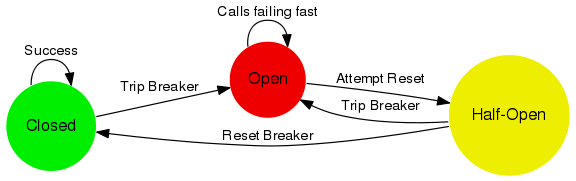
\includegraphics[width=0.75\textwidth]{images/circuit-breaker-states.png}
  \caption[Състояния на един прекъсвач на верига]{Състояния на един прекъсвач на верига (източник: \url{http://doc.akka.io/docs/akka/snapshot/common/circuitbreaker.html})}
  \label{fig:circuit-breaker-states}
\end{figure}

Akka предоставя имплементация на шаблона:

\begin{lstlisting}[texcl=true]
val breaker = CircuitBreaker(system.scheduler, 
                maxFailures = 10, 
                callTimeout = 20.seconds, 
                resetTimeout = 1.minute)

...

// При извикване на услугата
val result: Future[Int] = breaker.withCircuitBreaker(
                            (serviceActor ? SomeMessage()).mapTo[Int])
\end{lstlisting}

Ако услугата е отзивчива и изпраща веднага отговор за грешка при натоварване, вместо да се изчаква таумаута да изтече, то прекъсвачат би се задействал още по-рано, с което да ограничи излишното натоварване към услугата, както и да уведоми потребителите още по-рано, тъй като те също очакват нашия резултат. Така реактивността на системата се разпространява през всички нейни части, но само ако и те са реактивни.

\subsection{Връзка с неактьорски системи. Проактор чрез актьори}

Актьорският модел приема, че всичко се състои от актьори. Затова можем да приемем всяка една външна система за актьор, въпреки че не имплементира актьорските интерфейси от библиотеката, която използваме. За целта можем да дефинираме специален актьор, който да говори с нея и който да обвива нейния интерфейс. Така комуникацията със системата ще бъде енкапсулирана в актьора.

Като пример нека да обвием проактора, който реализирахме, във актьори. Нека дефинираме актьор \code{TcpManager}, който ни позволява да отваряме както сървърни канали, така и връзки към външни сървъри. Актьорът може да приема следните съобщения:

\begin{lstlisting}
object TcpManagerProtocol {
  case class Bind(address: InetSocketAddress)
  case class Connect(address: InetSocketAddress)
}
\end{lstlisting}

Нека приемането на някое от съобщенията да води до създаване на нов актьор, който да обработва новия канал и който да осъществява комуникацията с \emph{иницииращия} актьор. \code{TcpManager} актьорът и тези помощни актьори енкапсулират изцяло функционалността на проактора. Помощните актьори ще влязат в ролята на събитиен наблюдател (\englishterm{completion handler}). И ще уведомяват свързания с тях актьор за всяко събитие. Остава да се имплементира и събитийния диспечър, който просто изпраща съобщението от проактора към наблюдаващия актьор:

\begin{lstlisting}
object ActorCompletionDispatcher extends CompletionDispatcher[ActorRef] {
  def dispatch(message: Message, receiver: ActorRef): Unit =
    receiver ! message
}
\end{lstlisting}

Така имплементацията става следната:

\lstinputlisting[
  style=listing,
  firstline=8,
  caption={Енкапсулация на проактор чрез актьори}
]{../source/reactor-proactor/src/proactor/actors/manager/TcpManager.scala}

Актьорът, управляващ TCP връзките, изчаква връзката да се отвори и неговия наблюдател да се инициира, след което очаква явно да приеме актьорът, който ще я използва (това е полезно за връзки, създадени от сървърен канал). Примерът показва как един актьор може да премине през няколко състояния при своята инициализация.

Ехо сървър може да бъде имплементиран лесно:

\lstinputlisting[
  style=listing,
  firstline=11,
  caption={Актьорски ехо сървър}
]{../source/reactor-proactor/src/proactor/actors/ActorEchoServer.scala}

Така реализирахме проактор, който за потребителите на системата е изцяло съставен от актьори. Пълният код може да се види в \shortlabeledref{приложение}{att:reactor-proactor}.

\subsection{Реактивна класификация на актьорите}

Актьорите поддържат силно реактивните принципи. Базират се на асинхронни и неблокиращи съобщения, които могат да контролират напълно свободно. Скалират както вертикално така и хоризонтално, предоставят дистрибутирана комуникация, като за разлика от останалите инструменти в главата могат да бъдат размножавани от една система в друга. Това може да се използва за постигане на еластичност. Актьорите също така са лесно съвместими с различни механизми за осигуряване на устойчивост, като \englishterm{supervisor}, прекъсвач на веригата, скрито от другите актьори, рестартиране. Освен това лесно поддържат следене на времето на отговор на съобщенията и генериране на грешки, ако се забавят, което подобрява отзивчивостта.

\section{Процесни алгебри. Комуникиращи последователни процеси}

Съществуват различни процесни алгебри за конкурентни процеси, като $\pi$-смятането, CSP, CCS и други. Тук ще разгледаме комуникиращите последователни процеси (\englishterm{Communicating Sequential Processes, CSP}), въведени от Тони Хор \cite{hoare1978CSP}.

CSP системите се състоят от \emph{конкурентни процеси}, комуникиращи помежду си чрез \emph{канали}. За разлика от актьорите, тези процеси нямат адреси, а за да комуникират помежду си трябва да имат достъп до един и същ канал. Това води до по-слаба свързаност между тях. Изпращането и получаването на съобщение по канала обаче е синхронно и блокиращо. Изпращащия/приемащия процес блокират докато не се появи отсрещен такъв. В някои имплементации е възможно използването на опашки, които позволяват по-бавният от производителя и консуматора да не блокира.

Имплементациите на CSP в действителност не блокират физически нишки или други ресурси. Процесите представляват леки примитиви, които, подобно на актьорите, се изпълняват върху множество от нишки. Блокирането върху канал води до обработка на друг процес от нишката. Подобно на актьорите, останали без съобщения, процеса ще бъде продължен при пристигане на отсрещен процес.

Съществуват няколко популярни имплементации на CSP. Това са езиците occam и Go и библиотеката \code{core.async} за езика Clojure. Те обаче не имплементират напълно някои съществени математически свойства на CSP, като предвидимост на възможността за \englishterm{deadlock}.
\subsection{Реактивна класификация на CSP}

CSP са синхронни и блокиращи, но асинхронни и неблокиращи от гледна точка на изпълняващата ги нишки. Комуникират помежду си чрез явни единични съобщения, но блокиращо, което не предоставя гъвкавостта на асинхронните съобщения. Не предоставят механизъм за устойчивост. Скалират добре вертикално, но не могат да бъдат използвани дистрибутирано между няколко машини. Когато каналите се използват с ограничени опашки благодарение на блокирането се получава автоматичен механизъм за обратен натиск при препълване на опашката (повече в \shortlabeledref{секция}{sec:reactive-streams-with-backpressure})

CSP по-трудно се вписва с останалите реактивни средства, поради което тук няма да го разглеждаме подробно.

\section{Реактивни потоци}
\label{sec:reactive-streams}

Друга важна конструкция при реактивните системи е контролираното поточно предаване на съобщения като данни. В тази секция ще разгледаме различни имплементации и особености на такива абстракции.

\subsection{Изграждане на функционални потоци чрез \englishterm{Iteratee}}
\label{sec:iteratee}

Традиционния императивен подход за консумиране на даден източник на елементи е явното им извличане (\englishterm{pull}) един по един, реализирано от шаблона \emph{итератор}. Това обаче има няколко проблема:

\begin{itemize*}
  \item извличането представлява явен страничен ефект, извършван от консуматора. При използване на итератори всеки итератор има състояние, което бива контролирано от своя консуматор.
  
  \item поради страничните ефекти, състоянието и произволността консуматорите е трудно да бъдат композирани един с друг.
  
  \item единственият начин да се освободи входният ресурс е чрез неговото явно затваряне при завършване или възникване на грешка което често бива пропуснато.
\end{itemize*}

Нека да разгледаме алтернативен модел, при който производителите публикуват (\englishterm{push}) данни към консуматорите веднага щом те бъдат произведени. Това ни позволява да моделираме консуматорите като машина на състоянията, преминаваща към ново състояние при всеки вход от производителя. Този тип консуматор може да бъдат реализирам по чисто функционален начин. Нещо повече, в \shortlabeledref{глава}{ch:functional-programming} използвахме на няколко пъти методът \code{foldLeft}, който извършва именно това:

\begin{lstlisting}
def foldLeft[B](z: B)(f: (B, A) => B): B
\end{lstlisting}

Методът приема начално състояние и функция, която от текущото състояние и следващия елемент дава следващото състояние, като накрая резултатът е последното. За разлика от извличащият модел, тук, когато производителя може да произведе елементите си без странични ефекти (като при колекциите например), той също остава чисто функционален.	

Ще разгледаме абстракция, наречена \englishterm{iteratee}, която в основата си се базира на тази идея, като допълнително позволява преждевременно прекъсване на консумацията поради достигане на желан резултат или грешка, свързване с няколко източника и композиране на различни консуматори. Абстракцията е въведена от Олег Кисельов за езика Haskell през 2008-та година \cite{kiselyov2008Streams, kiselyov2012Iteratee}. Тук ще разгледаме имплементации, базирана на версията, описана от Джон Лато в \cite{lato2010Iteratee}.

\subsubsection{Синхронна реализация}

Първо ще разгледаме версия със синхронни източници и консуматори. Нека да реализираме тип, представляващ вход към консуматора:

\begin{lstlisting}
sealed trait Input[+I]
case class El[+I](value: I) extends Input[I]
case object Empty extends Input[Nothing]
case object EOF extends Input[Nothing]
\end{lstlisting}

Освен вход със следващ елемент \code{El[I]} ще разгледаме още два типа вход, означаващи специални състояния. Единият е \code{EOF} за достигнат край на входния поток. Другият е \code{Empty}, означаващ липса на нов вход. Той ще бъде използван за улесняване на имплементациите на места. При по-специални входни системи бихме могли да добавим и други специални типове.

Нека сега да видим как ще изглежда нашия консуматор, който ще наречем \englishterm{iteratee}:

\begin{lstlisting}
sealed trait Iteratee[I, +O]
case class Done[I, +O](value: O, rest: Input[I]) extends Iteratee[I, O]
case class Error[I, +O](error: Throwable) extends Iteratee[I, O]
case class Cont[I, +O](k: Input[I] => Iteratee[I, O]) extends Iteratee[I, O]
\end{lstlisting}

\code{Iteratee} е обект в три възможни състояния — \code{Done}, \code{Error} и \code{Cont}, моделиращ \emph{краен автомат}. Всяко \englishterm{iteratee} консумира вход от тип \code{I} докато не генерира единичен изход от тип \code{O}. Консуматорът може да приема вход докато се намира в състояние \code{Cont}. Това състояние дефинира функция \code{k}, която изчислява новото състояние на консуматора при вход на нов елемент. Можем да забележим, че това ново състояние не се запазва в обекта на консуматора и не води до странични ефекти, ами бива върнат като резултат от функцията. Нещо повече, обектът с предишното състояние може свободно да бъде използван с произволен брой други източници, генерирайки независими нови състояния. Това ни позволява да работим с консуматорите с като напълно неизменяеми обекти и да се възползваме от ползите от това.

Другите две състояния са крайните състояния на автомата, съответващи на успех с генерирана изходна стойност и на грешка. Ще поставим ограничение, че веднъж попаднали в крайните състояния \englishterm{iteratee} консуматорите не могат да излязат от тях. \code{Done} състоянието генерира и още един важен елемент — \code{rest}. Понякога е възможно входните елементи да бъдат консумирани само частично (например когато всеки елемент е цял масив от данни). Тогава \code{rest} представлява неконсумираната част на елемента. Това ни позволява да композираме различни \englishterm{iteratee} консуматори, без опасност от частична загуба на данни. Ще видим това малко по-късно в секцията.

Ще искаме при получаване на \code{EOF} консуматорът да преминава в крайно състояние, грешка при недостатъчен вход и успех с резултат иначе. Така можем да добавим методи за преминаване към крайно състояние \code{end} и за извличане на резултат:

\begin{lstlisting}
sealed trait Iteratee[I, +O] {
  def end = this match {
    case Cont(k) => k(EOF)
    case i => i
  }
  
  def run: Try[O] = this.end match {
    case Done(value, _) => Success(value)
    case Error(error) => Failure(error)
    case _ => Failure(new IllegalStateException("Diverging iteratee"))
  }
}
\end{lstlisting}

Нека за пример напишем имплементации на \englishterm{iteratee} консуматори — познатият ни вече \code{fold}, \code{sum}, генериращ сумата на всички елементи от входния поток, \code{take(n: Int)}, консумиращ първите до \code{n} елемента, и \code{foreach}, извършващ странични ефекти за всеки елемент:

\begin{lstlisting}
def fold[I, O](initial: O)(f: (O, I) => O): Iteratee[I, O] = {
  def step(state: O): Input[I] => Iteratee[I, O] = {
    case El(e) => Cont(step(f(state, e)))
    case Empty => Cont(step(state))
    case EOF => Done(state, EOF)
  }
  Cont(step(initial))
}

val sum = fold[Int, Int](0)(_ + _)

def take[A](n: Int): Iteratee[A, List[A]] = {
  def step(elements: List[A]): Input[A] => Iteratee[A, List[A]] = {
    case El(e) if elements.size == n - 1 =>
      Done((e :: elements).reverse, Empty)
    case El(e) => Cont(step(e :: elements))
    case Empty => Cont(step(elements))
    case EOF => Done(elements.reverse, EOF)
  }
  Cont(step(Nil))
}

def foreach[I](f: I => Unit): Iteratee[I, Unit] = {
  def step: Input[I] => Iteratee[I, Unit] = {
    case El(e) => f(e); Cont(step)
    case Empty => Cont(step)
    case EOF => Done((), EOF)
  }
  Cont(step)
}
\end{lstlisting}

Можем да видим, че реализираните консуматори съответстват на функционалните абстракции, които разгледахме в \shortlabeledref{глава}{ch:functional-programming} и по-специално на тези, генериращи единичен резултат. С разгледаните в тази секция абстракции ще искаме именно да си върнем композитността на разгледаните в главата функции от по-висок ред, но приложени за потоци от данни. Реализацията на \code{sum} е именно чрез друг консуматор, скриващ инцидентната сложност.

Нека да моделираме и самите източници (производители), които ще наречем \englishterm{enumerator}. Тяхната роля е да публикуват елементите си към консуматорите до достигане на крайно състояние или до изчерпване на източника:

\begin{lstlisting}
trait Enumerator[I] {
  def apply[O](iteratee: Iteratee[I, O]): Iteratee[I, O]
}
\end{lstlisting}

Методът \code{apply} заменя метода \code{foldLeft}, който видяхме в началото на секцията, но с желаното от нас допълнително поведение.

Да разгледаме имплементация за колекции:

\begin{lstlisting}
object Enumerator {
  def apply[T](values: T*) = new Enumerator[T] {
    @tailrec
    private def enumerate[O](values: Seq[T], iteratee: Iteratee[T, O]): Iteratee[T, O] = iteratee match {
      case Cont(k) if !values.isEmpty =>
        enumerate(values.tail, k(El(values.head)))
      case _ => iteratee
    }
  
    def apply[O](iteratee: Iteratee[T, O]): Iteratee[T, O] =
      enumerate(values, iteratee)
  }
}

Enumerator(1, 2, 3, 4, 5, 6)(Iteratee.sum).run // Success(21)
\end{lstlisting}

Можем да видим как завършването на консумацията веднага прекъсва публикуването на елементи. Така ако \englishterm{enumerator} обекта взима данните от източник, който трябва да бъде затворен (файл, сокет или друго), то затварянето би станало автоматично веднага при достигане на крайно състояние, без притеснение, че може да бъде забравено.

\subsubsection{Композитност}

При така реализираните абстракции лесно можем да добавим монадна композитност:

\begin{lstlisting}
sealed trait Iteratee[I, +O] {
  def map[B](f: O => B): Iteratee[I, B] = this match {
    case Done(value, rest) => Done(f(value), rest)
    case Cont(k) => Cont(i => k(i) map f)
    case Error(e) => Error(e)
  }
  
  def filter(f: O => Boolean): Iteratee[I, O] = this match {
    case done@Done(value, rest) =>
      if (f(value)) done
      else Error(new NoSuchElementException)
    case it => it
  }
  
  def flatMap[B](f: O => Iteratee[I, B]): Iteratee[I, B] = this match {
    case Done(value, rest) => f(value) match {
      case Done(_, El(_)) => Error(
        new IllegalStateException("Invalid initial iteratee state"))
      case Done(valueB, _) => Done(valueB, rest)
      case Cont(k) => k(rest)
      case Error(e) => Error(e)
    }
    case Cont(k) => Cont(i => k(i) flatMap f)
    case Error(e) => Error(e)
  }
}

object Iteratee {
  implicit def iterateeMonad[I] = new MonadWithZero[({type f[+O] = Iteratee[I, O]})#f] {
    def mzero[A]: Iteratee[I, A] = Error(new NoSuchElementException)
    def flatMap[A, B](m: Iteratee[I, A])(f: (A) => Iteratee[I, B]): Iteratee[I, B] = m flatMap f
    def unit[A](a: => A): Iteratee[I, A] = Done(a, Empty)
    
    override def map[A, B](m: Iteratee[I, A])(f: (A) => B): Iteratee[I, B] = m map f
  }
}
\end{lstlisting}

В \shortlabeledref{приложение}{att:iteratees} може да се види имплементацията и за \code{Enumerator}. 

Монадната композиция на \englishterm{enumerator} е като тази при списъците и колекциите, която разгледахме в \shortlabeledref{глава}{ch:functional-programming}. Интересна е монадната композиция на \englishterm{iteratee}:

\begin{lstlisting}
for {
  List(a, b) <- take(2)
  _ <- drop(a)
  c <- sum
} yield (a, b, c)
\end{lstlisting}

\code{take} и \code{sum} за вече разгледаните \englishterm{iteratee} консуматори, а \code{drop} пропуска \code{n} на брой елемента от входния поток. Можем да видим, че при копозирането на \englishterm{iteratee} обекти всеки от тях се прилага последователно към вход до завършването си, като всеки може да зависи от резултата на предходния — първо се взимат два елемента, пропускат се \code{a} на брой и се взима сумата на останалите елементи, генерирайки тройката \code{(a, b, c)}. Това може да е доста мощен механизъм.

\code{Enumerator} обектите могат да се композират и немонадно като конкатенация на потоците. За целта е реализирана операция \code{andThen}.

\begin{lstlisting}
(Enumerator(1, 2, 3) andThen Enumerator(4, 5))(sum).run // Success(15)
\end{lstlisting}

\subsubsection{Трансформации на входния поток}

Реализирахме преизползваеми консуматори \code{fold}, \code{sum}, \code{foreach} и др., които генерират единичен резултат. Нека да видим как да реализираме и друг тип стандартни функционални преобразувания, а именно трансформиращите самия поток. За целта ще въведем абстракцията \englishterm{enumeratee}:

\begin{lstlisting}
trait Enumeratee[U, V] {
  def apply[O](iteratee: Iteratee[V, O]): Iteratee[U, Iteratee[V, O]]
}
\end{lstlisting}

\code{Enumeratee} обвива в себе си подаденото \code{iteratee}, трансформирайки потока, преди да го препрати към \code{iteratee}. Резултатът ново \code{Iteratee}, чийто изход е последното състояние на подаденото \code{iteratee}.

Чрез тази абстракция лесно могат да бъдат реализирани трансформатори като \code{map} и \code{filter}, кодът на които може да бъде видян в \shortlabeledref{приложение}{att:iteratees}. За лесно използване на \code{Enumeratee} ще напишем помощни функции за прикачване към \code{Enumerator} или \code{Iteratee}:

\begin{lstlisting}
trait Enumerator[I] { self =>
  def through[T](enumeratee: Enumeratee[I, T]): Enumerator[T] = new Enumerator[T] {
    def apply[O](iteratee: Iteratee[T, O]): Iteratee[T, O] = self(enumeratee(iteratee)).end match {
      case Done(i, _) => i
      case Error(e) => Error(e)
      case _ => Error(
        new IllegalStateException("Unexpected Enumeratee state"))
    }
  }
}

trait Enumeratee[U, V] {
  def transform[O](iteratee: Iteratee[V, O]): Iteratee[U, O] = this(iteratee) flatMap {
    case Done(value, _) => Done(value, Empty)
    case Error(e) => Error(e)
    case Cont(k) => k(EOF) match {
      case Done(value, _) => Done(value, Empty)
      case Error(e) => Error(e)
      case Cont(k) => Error(new IllegalStateException("Diverging iteratee"))
    }
  }
}
\end{lstlisting}

Следващите редове са еквивалентни:

\begin{lstlisting}
(Enumerator(1, 2, 3, 4, 5) through Enumeratee.map(_ * 2) through Enumeratee.filter(_ > 2))(Iteratee.sum)
(Enumerator(1, 2, 3, 4, 5))(Enumeratee.map[Int, Int](_ * 2) transform (Enumeratee.filter[Int](_ > 2) transform Iteratee.sum))
\end{lstlisting}

Ако въведем символни псевдоними \code{|>>} за \code{Enumerator.apply}, \code{&>} за \code{Enumerator.through} и \code{&>>} за \code{Enumeratee.transform}, то предните редове могат да се запишат по-ясно като:

\begin{lstlisting}
import Enumeratee._
Enumerator(1, 2, 3, 4, 5) &> map(_ * 2) &> filter(_ > 2) |>> Iteratee.sum
Enumerator(1, 2, 3, 4, 5) |>> map[Int, Int](_ * 2) &>> (filter[Int](_ > 2) &>> Iteratee.sum)
\end{lstlisting}

Така ясно се вижда през какви етапи минава потокът.

Друга интересна трансформация е \code{grouped}. Тя приема \code{Iteratee}, като прекарва входния поток през него, докато не произведе стойност, след което бъде рестартирано за нов вход. Всяка произведена стойност образува поток, който е резултатът от трансформацията. Това е възможно благодарение на неизменяемата природа на тези абстракции. Да разгледаме пример:

\begin{lstlisting}
val asciiLineChunked: Iteratee[Array[Byte], String] = {
  def toString(chunks: List[Array[Byte]]) = new String(
    Array.concat(chunks.reverse: _*), "US-ASCII")
  
  def step(chunks: List[Array[Byte]]): Input[Array[Byte]] => Iteratee[Array[Byte], String] = {
    case Empty => Cont(step(chunks))
    case EOF => Done(toString(chunks), EOF)
    case El(chars) => chars.span(_ != '\n') match {
      case (_, Array()) => Cont(step(chars :: chunks))
      case (lineEnd, rest) =>
        Done(toString(lineEnd :: chunks), El(rest.tail))
    }
  }
  Cont(step(List.empty))
}.map(_.stripSuffix("\r"))

val lines = Enumeratee.grouped(asciiLineChunked)
\end{lstlisting}

\code{asciiLineChunked} е консуматор на масиви от байтове, консумиращ един ред (в \emph{ASCII encoding}) от тях. Прилагайки \code{grouped} получаваме \englishterm{enumeratee} трансформатор на поток от масиви от байтове към поток от редове. Тук предаваме входа на масиви, вместо байт по байт, за постигане на по-голяма ефективност, поради което е необходимо да се възползваме от \code{rest} параметъра на \code{Done}.

\subsubsection{Монадна реализация}

\englishterm{Iteratee} абстракциите, които разгледахме, биха станали по-полезни ако могат да се комбинират с монадни ефекти. За целта ще изменим вида им по следния начин:

\begin{lstlisting}
sealed trait Step[I, O, F[_]]
case class Done[I, O, F[_]](value: O, rest: Input[I]) extends Step[I, O, F]
case class Error[I, O, F[_]](error: Throwable) extends Step[I, O, F]
case class Cont[I, O, F[_]](k: Input[I] => Iteratee[I, O, F]) extends Step[I, O, F]

trait Iteratee[I, O, F[_]] {
  def value: F[Step[I, O, F]]
}

trait Enumerator[I, F[_]] {
  def apply[O](iteratee: Iteratee[I, O, F]): Iteratee[I, O, F]
}

trait Enumeratee[U, V, F[_]] {
  def apply[O](iteratee: Iteratee[V, O, F]): Iteratee[U, Iteratee[V, O, F], F]
}
\end{lstlisting}

Възможните състояние са изведени отделно в \code{Step} обекти. Параметърът \code{F} определя монадата, която ще бъде използвана. Така типът \code{Iteratee} представлява стъпка, скрита зад монаден ефект. Това позволява на \code{Enumerator} също да работи с монадни източници от тип \code{F}.

Досегашните имплементации изискват известни изменения. Например можем да повдигнем синхронните \englishterm{iteratee} обекти в монадни чрез следната функция:

\begin{lstlisting}
object Iteratee {
  def apply[I, O, F[_]](step: Step[I, O, F])(implicit m: Monad[F]) = new Iteratee[I, O, F] {
    def value: F[Step[I, O, F]] = (m.unit(step))
  }
  
  def liftSimpleIteratee[I, O, F[_]](iteratee: simple.Iteratee[I, O])
  (implicit m: Monad[F]): Iteratee[I, O, F] = iteratee match {
    case simple.Done(value, rest) => Iteratee(Done(value, rest))
    case simple.Error(e) => Iteratee(Error(e))
    case simple.Cont(k) => Iteratee(
      Cont(input => liftSimpleIteratee(k(input))))
  }
}
\end{lstlisting}

Всички свойства, които разгледахме, остават същите и при монадната реализация.

В следващите части на дипломната работа ще използваме имплементацията на \englishterm{iteratee} от рамката Play. Тя се базира конкретно на \englishterm{future} монадата, което добавя асинхронност към потоците. В рамката типовете са дефинирани по следния начин:

\begin{lstlisting}
sealed trait Step[E, +A]
case class Done[+A, E](a: A, remaining: Input[E]) extends Step[E, A]
case class Cont[E, +A](k: Input[E] => Iteratee[E, A]) extends Step[E, A]
case class Error[E](msg: String, input: Input[E]) extends Step[E, Nothing]

trait Iteratee[E, +A] {
  def fold[B](folder: Step[E, A] => Future[B])
             (implicit ec: ExecutionContext): Future[B]
}

trait Enumerator[E] {
  def apply[A](i: Iteratee[E, A]): Future[Iteratee[E, A]]
}

trait Enumeratee[From, To] {
  def applyOn[A](inner: Iteratee[To, A]): Iteratee[From, Iteratee[To, A]]
}
\end{lstlisting}

Основната разлика е, че имплементацията на \code{Iteratee} се базира на метод \code{fold}, вместо на заключена зад монада стъпка. \code{folder} съдържа логиката на производителя, който публикува вход, като той трябва да извика \code{fold} метода при нов входен елемент за да получи текущата стъпка. \code{fold} може да извиква \code{folder} когато е готов за това. Допълнително методът приема обект \code{ExecutionContext}, който представлява изчислителната среда, в която да се изпълняват \code{Future} обектите. Видимостта на на елементите на потоците между различни нишки се гарантира именно чрез тях. Имплементацията предоставя подобни помощни обекти и функции, като тези които разгледахме, като допълнително приемат среда, в която да се изпълнява тяхната логика.

\subsubsection{Парсър на HTTP съобщения чрез \englishterm{iteratee}}

Чрез разгледаните абстракции много лесно може да реализирам чисто функционален краен автомат за парсване на HTTP съобщения, съставен чрез композиране на малки части:

\lstinputlisting[
  style=listing,
  firstline=8,
  caption={Функционален парсър на HTTP съобщения}
]{../source/web-server/src/http/HttpMessageIteratee.scala}

В имплементацията парсването ясно се разделя на парсване на началния ред, парсване на \englishterm{header} стойностите и парсване на тялото на съобщението, които комбинирани заедно дават HTTP съобщение (редове 49 до 59). Първите две разглеждат входа като ASCII редове, докато парсването на тялото директно чете байтовете.

\subsubsection{Връзка с външен вход/изход. Връзка с актьори}

Потоците ни позволяват да отделим вход и изход до най-външните точки на програмата, като логиката към тях да минава през функционалните потоци. За целта може да реализираме наблюдател към нашия реактор, който да приема двойка \code{Iteratee} и \code{Enumeratee} обекти. Всеки вход към канала ще бъде предаван към \code{Iteratee} обекта, а всяка стойност, публикувана от \code{Enumeratee} обекта ще бъде извеждана като изход в канала. Този наблюдател има следния вид и неговата реализация може да бъде видяна в \shortlabeledref{приложение}{att:web-server}:

\begin{lstlisting}
class IterateeHandler(reactor: FullReactor, channel: SocketChannel)
  (in: Iteratee[Array[Byte], _], out: Enumerator[Array[Byte]])
  extends Handler with CloseOnIOError
\end{lstlisting}

Така може да имплементираме следния ехо сървър, приемащ UTF-8 текст, който допълнително трансформира входа си към главни букви:

\begin{lstlisting}
object IterateeUppercaseEchoServer {
  def main (args: Array[String]): Unit = {
    new WorkersServer(8000)((reactor, channel) => {
      val (in, inputEnum) = Concurrent.joined[Array[Byte]]
      val out = inputEnum &>
                CharEncoding.decode("UTF-8") &>
                Enumeratee.map(_.toUpperCase.getBytes("UTF-8"))
      new IterateeHandler(reactor, channel)(in, out)
    }).start()
  }
}
\end{lstlisting}

\code{CharEncoding} декодира входа, следейки например за когато една буква е разделена между два входни масива. Ключовото тук е \code{Concurrent.joined} функцията. Тя връща двойка \code{(Iteratee, Enumerator)}, като всеки вход към \englishterm{iteratee} елемента се преобразува към елемент на \englishterm{enumerator} производителя. Това позволява изграждане именно на такива цялостни потоци от входа до изхода. Ще отбележим още, че тъй като вече \englishterm{iteratee} обектите приемат вход асинхронно, то на всеки нов вход реакторния наблюдател спира регистрация за четене докато входа не бъде приет. Така ако консуматора е бавен се оказва обратен натиск на канала, което се поддържа автоматично от TCP протокола.

Друга интересна връзка, която може да бъде направена, е имплементация на \englishterm{enumeratee} чрез актьор, който да преобразува потока.

\subsection{Други поточни имплементации. \englishterm{Akka Streams}}

През годините в Haskell средите се развиват различни библиотеки, базирани на идеята за \englishterm{iteratee} абстракции, но с цел да се опрости тяхното използване. Такава е например библиотеката \englishterm{Machines} за Haskell, на която която се базира и имплементация за скала в библиотеката \englishterm{scalaz-stream}.

Друга интересна имплементация е в Akka разширението \englishterm{Akka Streams} \cite{akkaStreams2015}. Библиотеката предоставя интерфейс за изграждане на поточни графи по функционален начин, като всеки граф след това бива „материализиран“ до актьори, изграждащи реалния поток, което дава автоматично скалиране и паралелизъм. Библиотеката предоставя различни видове възли, с които да бъде изграден графа. Те се различават по входовете и изходите, които имат, и логиката, която енкапсулират. Основните възли са \code{Source}, \code{Flow} и \code{Flow}, които съответстват на разгледаните \englishterm{enumerator}, \englishterm{enumeratee} и \englishterm{iteratee}. Потоците от \englishterm{Akka Streams} също могат да произвеждат крайни резултати и също могат да бъдат интегрирани с \englishterm{future} обекти или входно/изходни реализации. Библиотеката \englishterm{Akka HTTP} предоставя връзка с HTTP услуги, а \englishterm{Akka IO} на TCP ниво.

\englishterm{Akka Streams} набляга също така на контролирането на буферирането и на обратния натиск. Ще разгледаме това в следващата подсекция.

\subsection{Реактивни потоци с обратен натиск}
\label{sec:reactive-streams-with-backpressure}

\englishterm{Reactive streams} \cite{reactiveStreamsSpecification2015} е инициатива на организациите \englishterm{Typesafe, Twitter, Netflix, Red Hat} и др. от 2014-та и 2015-та година за стандартизиране на общ интерфейс между различни асинхронни поточни имплементации върху публикуващ (\englishterm{push}) модел с явна поддръжка на контролиране на потока от консуматора чрез обратен натиск по извличащ (\englishterm{pull}) модел. Интерфейсът е на ниско ниво, базиран на \englishterm{publish-subscribe} подход и използващ \englishterm{callback} механизъм. Целта на това е лесно да може да бъде имплементиран от различните библиотеки. \shortlabeledref{Фигура}{fig:reactive-streams} представя компонентите на Java спецификацията.

\begin{figure}
  \centering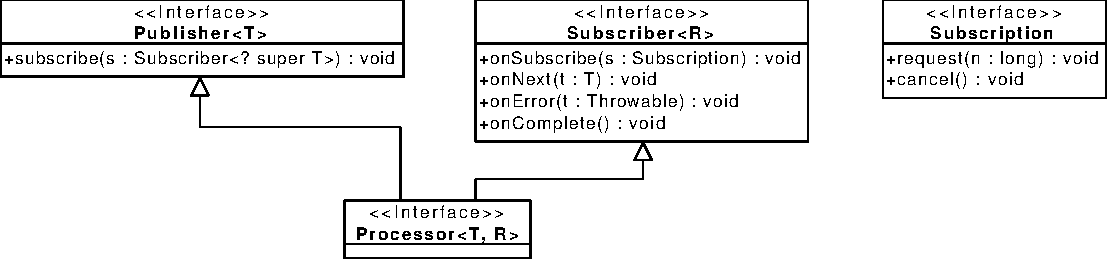
\includegraphics[width=\textwidth]{images/reactive-streams.pdf}
  \caption{Компоненти на реактивните потоци с обратен натиск}
  \label{fig:reactive-streams}
\end{figure}

Отново може да открием съответствие между \code{Publisher}, \code{Processor} и \code{Subscriber} и \englishterm{enumerator}, \englishterm{enumeratee} и \englishterm{iteratee}. Методите на всички интерфейси могат да бъдат извиквани асинхронно и имплементациите трябва да гарантират многонишковата комуникация и безопасност в такива случаи. \code{Subscribe} обектите, подобно на \englishterm{iteratee} потоците, приемат като вход следващ елемент и сигнал за край на потока, като в допълнение приемат сигнал за иницииране и сигнал за грешка в производителя. \code{Publisher} обектите публикуват поточните елементи към регистриралите се \code{Subscriber} обекти по \englishterm{push} модел. Всеки един консуматор би следвало да има буфер, в който да трупа елементи за обработка. Както видяхме в \shortlabeledref{глава}{ch:reactive-programming-principles} тази опашка трябва да е ограничена и тя или ще е близо до празна, което значи, че консуматорът работи бързо и елементите могат да бъдат публикувани без проблем, или близо до пълна, което значи, че консуматорът е бавен и трябва да започне изхвърляне на новодошли съобщения (елементи). Затова ключовото в спецификацията е \code{Subscription} обекта, чрез който консуматора може да контролира производителя. Всеки път когато консуматорът освободи място в своя буфер той трябва да извика \code{request} метода с брой елементи, който да е достатъчен за да се поберат в буфера. Производителят няма право да изпраща повече елементи от това, което е било поискано. Така реализацията става комбинация между публикуващ (\englishterm{push}) и извличащ (\englishterm{pull}) модел, като при бърз консуматор се доближава до публикуващия, а при бавен до извличащия.

Обратния натиск ни гарантира, че буферът няма да се препълни или няма да бъде запълнена паметта на системата. Така получаваме по-добра устойчивост. Допълнително намаляваме излишния трафик по мрежата когато системата е натоварена. Липсата на това би могло да доведе и до срив на мрежата. Друго важно свойство е, че обратния натиск се разпространява обратно по цялата верига. Ако потокът е изграден от няколко междинни трансформиращи възела, тоест \code{Processor} обекти, то натискът от крайния консуматор се отразява на всеки от производителите по веригата. Така потока е бърз колкото най-бавната си част.

Подобен механизъм е имплементиран и в TCP протокола. При него се поддържа буфер, наречен \emph{прозорец}, който се свива и разширява, в зависимост от скоростта на потока, и се реализира обратен механизъм за потвърждаване на пристигналите данни за следене и контрол. Така реактивните потоци позволяват този контрол да бъде пренесен към програмната логика, което обикновено липсва при повече съвременни системи. Така реактивните системи могат да контролират скоростта на всеки един TCP поток, без да са заплашени от претоварване от него. Имплементацията, която направихме в \shortlabeledref{секция}{sec:iteratee} за поточна връзка с външен вход/изход имаше именно такъв контрол над TCP канала.

\englishterm{Akka Streams} библиотеката имплементира спецификацията, като предоставя добър контрол на използваните буфери и обратния натиск, включително върху TCP потоците. \emph{Iteratee} абстракциите също предоставят естествен контрол, тъй като при тях производителят не може да публикува елемент, преди консуматора да е готов с консумирането на предишния — изчаква върнатия от него \code{Future} обект да завърши. Това теоритично значи, че те имат буфер от един елемент, но би могло да се използва специален \englishterm{enumeratee} обект, който да извършва буфериране, както и самите елементи да се изпращат на масиви, както направихме при парсването на редове. Play рамката предоставя имплементация на спецификацията за \englishterm{iteratee}. Друго съществуващи имплементации са за библиотеката RxJava, за базата MongoDB, за релационната библиотека Slick и други. Така софтуерни компоненти от най-различен тип могат да комуникират помежду си поточно.

\subsection{Функционално реактивно програмиране}

Функционалното реактивно програмиране (\englishterm{FRP}) е модел за вариращи във времето стойности, дефиниран от Конал Елиът \cite{elliott2009PushPullFRP}. Моделът дефинира две основни абстракции — поведения и събития. Поведенията са непрекъснати във времето стойности, а събитията поток от дискретни стойности, дефинирани за определен момент от времето. Така поведенията представляват функция на момент във времето, а събитията списък от двойки (момент, стойност):

\begin{lstlisting}
type Behaviour[A] = Time => A
type Event[A] = List[(Time, A)]
\end{lstlisting}

Едно поведение има стойност във всеки един момент, а един събитиен поток само за определни моменти. FRP не дефинира как тези абстракции да бъдат реализирани, но дефинира функционални операции за тяхното трансформиране и композиране, резултатът от които е нови поведения и събития, от където идва реактивността им. Зависимостта единствено от времето означава, че тези трансформации се извършват единствено синхронно и едновременно. Нека първо да разгледаме основните операции и примитиви.

Основното поведение, на което се базират всички останали, е времето: 

\begin{lstlisting}
val time: Behaviour[Time] = identity
\end{lstlisting}

Операциите върху абстракциите биват дефинирани чрез денотационна семантика, използвайки познати типове на класове. Така за поведенията се дефинират вече познатите ни монадни, апликативни и функторни (т.е. наличие на \code{map}) операции. За събитията освен тях биват дефинирани още моноидни операции за сливане на два събитийни потока. Точната дефиниция може да бъде видяна в \cite{elliott2009PushPullFRP}. Освен това се дефинира операция за композиране на поведения и потоци \code{switcher}

\begin{lstlisting}
def switcher[A](b0: Behaviour[A], e: Event[Behaviour[A]]): Behaviour[A] =
  (t: Time) => (b0 :: e.filter({ case (time, _) =>  time < t})).last
  
def stepper[A](a: A, e: Event[A]): Behaviour[A] =
  switcher(Monad.unit(e), e.map(Monad.unit(_)))
\end{lstlisting}

Резултатът от операцията е поведение, което първоначално съвпада с поведението \code{b0}, но за всяко събитие в потока \code{e} променя стойността си с новото поведение от него. Чрез \code{switcher} може да бъде дефинирата по-простоата операция \code{stepper}.

Статията дефинира и абстракция \englishterm{future}, представляваща единично събитие във времето, тоест двойка \code{(Time, A)}. Това реално съответства на познатите ни \englishterm{future} обекти, но описани в този модел.

Имплементацията на тази семантика зависи от конкретната библиотека за FRP. Библиотеките не пазят списък със всички двойки в събитийните потоци и не съхраняват всички стойности на поведенията за всеки момент. Поради невъзможността за реализиране на непрекъснати стойности в съвременните компютри поведенията са симулирани чрез дискретни стойности (например в имплементациите времето може да бъде обновявано дискретно на интервали, като имплементацията може да оптимизира това да става само когато има нужда). Статията разглежда различни имплементационни детайли и подходи.

Този модел реално позволява създаването на граф от зависещи едни от други стойности и събитийни потоци, а именно \englishterm{dataflow} поток. Поради синхронната си природа е изключително подходящ за потребителски интерфейси, където състоянието се обновява синхронно в резултат на възникнали събития. За целта трябва да въведем събития и поведения, зависещи от външни странични ефекти. Такива са например поведение за текущата позиция на мишката или събития за кликване или натискане на бутон на клавиатурата. Аналогично стойностите на някои поведения може да се отразяват автоматично върху състоянието на потребителския интерфейс. Тези странични ефекти отново са ограничени в двата края на потока. Така добавихме асинхронен вход към модела, който бива обработен синхронно.

Съществуват най-различни реализации, най-често Haskell базирани, като \englishterm{Sodium} и \englishterm{reactive-banana}, но и други, като езикът \englishterm{Elm}. Някои реализации не следват стриктно модела и позволяват асинхронно обновяване, вместо синхронно. Това дава по-голяма гъвкавост, но може да доведе до временно невалидно състояние в потребителския интерфейс в някои случаи. Такива имплементации са \englishterm{Reactive Extensions (RxJava, RxJS и други)}, \englishterm{bacon.js}, \englishterm{kefir.js} и други.

\subsection{Реактивна класификация на потоците}

Потоците позволяват изграждането на големи графи от възли, разпространяващи си съобщения с различна скорост без блокиране, моделирайки \englishterm{dataflow} система. Асинхронните потоци скалират без проблем вертикално и хоризонтално, като дистрибутираната комуникация може да бъде извършена чрез явна входно/изходна връзка. Асинхронните потоци могат да поддържат механизъм за обратен натиск, който да ограничи получаваните съобщения с цел осигуряване на устойчивост. Всяка възникнала грешка бива разпространена в потока и той може да бъде автоматично прекъснат, без срив в системата.

\section{Обобщение на реактивните средства}

Чрез реализацията на уеб сървър, както и чрез други примери, видяхме, че реактивните средства всъщност се допълват помежду си, предоставяйки различни реактивни и функционални свойства. Някои от разгледаните имплементации дори се базираха на други. Всяко средство подпомага най-вече конкретни свойства на реактивните системи и правилното композиране води до реализация на всички от тях.
